\documentclass[12pt,twoside]{report}

%%%%%%%%%%%%%%%%%%%%%%%%%%%%%%%%%%%%%%%%%%%%%%%%%%%%%%%%%%%%%%%%%%%%%%%%%%%%%

% Definitions for the title page
% Edit these to provide the correct information
% e.g. \newcommand{\reportauthor}{Timothy Kimber}

\newcommand{\reporttitle}{A robot application with voice command}
\newcommand{\reportauthor}{Hong Anh Vu}
\newcommand{\supervisor}{Jim Cunningham \\ Stefan Leutenegger}
\newcommand{\degreetype}{Machine Learning}

\newcommand{\tbf}[1]{\textbf{#1}}
\newcommand{\tit}[1]{\textit{#1}}
\setlength{\parskip}{0.2cm}


%%%%%%%%%%%%%%%%%%%%%%%%%%%%%%%%%%%%%%%%%%%%%%%%%%%%%%%%%%%%%%%%%%%%%%%%%%%%%

% load some definitions and default packages
%%%%%%%%%%%%%%%%%%%%%%%%%%%%%%%%%%%%%%%%%
% University Assignment Title Page 
% LaTeX Template
% Version 1.0 (27/12/12)
%
% This template has been downloaded from:
% http://www.LaTeXTemplates.com
%
% Original author:
% WikiBooks (http://en.wikibooks.org/wiki/LaTeX/Title_Creation)
%
% License:
% CC BY-NC-SA 3.0 (http://creativecommons.org/licenses/by-nc-sa/3.0/)
% 
%
%%%%%%%%%%%%%%%%%%%%%%%%%%%%%%%%%%%%%%%%%
%----------------------------------------------------------------------------------------
%	PACKAGES AND OTHER DOCUMENT CONFIGURATIONS
%----------------------------------------------------------------------------------------
\usepackage[a4paper,hmargin=2.8cm,vmargin=2.0cm,includeheadfoot]{geometry}
\usepackage{textpos}
\usepackage{natbib} % for bibliography
\usepackage{tabularx,longtable,multirow,subfigure,caption}%hangcaption
\usepackage{fncylab} %formatting of labels
\usepackage{fancyhdr} % page layout
\usepackage{url} % URLs
\usepackage[english]{babel}
\usepackage{amsmath}
\usepackage{graphicx}
\usepackage{dsfont}
\usepackage{epstopdf} % automatically replace .eps with .pdf in graphics
\usepackage{backref} % needed for citations
\usepackage{array}
\usepackage{latexsym}
\usepackage[pdftex,pagebackref,hypertexnames=false,colorlinks]{hyperref} % provide links in pdf

\hypersetup{pdftitle={},
  pdfsubject={}, 
  pdfauthor={},
  pdfkeywords={}, 
  pdfstartview=FitH,
  pdfpagemode={UseOutlines},% None, FullScreen, UseOutlines
  bookmarksnumbered=true, bookmarksopen=true, colorlinks,
    citecolor=black,%
    filecolor=black,%
    linkcolor=black,%
    urlcolor=black}

\usepackage[all]{hypcap}
\usepackage[section]{placeins}

%\usepackage{color}
%\usepackage[tight,ugly]{units}
%\usepackage{float}
%\usepackage{tcolorbox}
%\usepackage[colorinlistoftodos]{todonotes}
% \usepackage{ntheorem}
% \theoremstyle{break}
% \newtheorem{lemma}{Lemma}
% \newtheorem{theorem}{Theorem}
% \newtheorem{remark}{Remark}
% \newtheorem{definition}{Definition}
% \newtheorem{proof}{Proof}


%%% Default fonts
\renewcommand*{\rmdefault}{bch}
\renewcommand*{\ttdefault}{cmtt}



%%% Default settings (page layout)
\setlength{\parindent}{0em}  % indentation of paragraph

\setlength{\headheight}{14.5pt}
\pagestyle{fancy}
\renewcommand{\chaptermark}[1]{\markboth{\chaptername\ \thechapter.\ #1}{}} 

\fancyfoot[ER,OL]{\sffamily\textbf{\thepage}}%Page no. in the left on odd pages and on right on even pages
\fancyfoot[OC,EC]{\sffamily }
\renewcommand{\headrulewidth}{0.1pt}
\renewcommand{\footrulewidth}{0.1pt}
\captionsetup{margin=10pt,font=small,labelfont=bf}


%--- chapter heading

\def\@makechapterhead#1{%
  \vspace*{10\p@}%
  {\parindent \z@ \raggedright \sffamily
    \interlinepenalty\@M
    \Huge\bfseries \thechapter \space\space #1\par\nobreak
    \vskip 30\p@
  }}

%---chapter heading for \chapter*  
\def\@makeschapterhead#1{%
  \vspace*{10\p@}%
  {\parindent \z@ \raggedright
    \sffamily
    \interlinepenalty\@M
    \Huge \bfseries  #1\par\nobreak
    \vskip 30\p@
  }}

\allowdisplaybreaks

\usepackage{siunitx}
\usepackage{graphicx}
%\usepackage{subcaption}
% load some macros
% Here, you can define your own macros. Some examples are given below.

\newcommand{\R}[0]{\mathds{R}} % real numbers
\newcommand{\Z}[0]{\mathds{Z}} % integers
\newcommand{\N}[0]{\mathds{N}} % natural numbers
\newcommand{\C}[0]{\mathds{C}} % complex numbers
\renewcommand{\vec}[1]{{\boldsymbol{{#1}}}} % vector
\newcommand{\mat}[1]{{\boldsymbol{{#1}}}} % matrix


\date{June 2017}

\begin{document}

% load title page
% Last modification: 2015-08-17 (Marc Deisenroth)
\begin{titlepage}

\newcommand{\HRule}{\rule{\linewidth}{0.5mm}} % Defines a new command for the horizontal lines, change thickness here


%----------------------------------------------------------------------------------------
%	LOGO SECTION
%----------------------------------------------------------------------------------------


\includegraphics[width = 4cm]{./figures/imperial}\\[0.5cm] 

\center % Center remainder of the page

%----------------------------------------------------------------------------------------
%	HEADING SECTIONS
%----------------------------------------------------------------------------------------

\textsc{\Large Imperial College London}\\[0.5cm] 
\textsc{\large Department of Computing}\\[0.5cm] 

%----------------------------------------------------------------------------------------
%	TITLE SECTION
%----------------------------------------------------------------------------------------

\HRule \\[0.4cm]
{ \huge \bfseries \reporttitle}\\ % Title of your document
\HRule \\[1.5cm]
 
%----------------------------------------------------------------------------------------
%	AUTHOR SECTION
%----------------------------------------------------------------------------------------

\begin{minipage}{0.4\textwidth}
\begin{flushleft} \large
\emph{Author:}\\
\reportauthor % Your name
\end{flushleft}
\end{minipage}
~
\begin{minipage}{0.4\textwidth}
\begin{flushright} \large
\emph{Supervisor:} \\
\supervisor % Supervisor's Name
\end{flushright}
\end{minipage}\\[4cm]


%----------------------------------------------------------------------------------------
%	FOOTER & DATE SECTION
%----------------------------------------------------------------------------------------
\vfill % Fill the rest of the page with whitespace
This interim document is a contribution toward a full report to be 
submitted in partial fulfillment of the requirements for the MSc degree in
\degreetype~of Imperial College London\\[0.5cm]

%Submitted in partial fulfillment of the requirements for the MSc degree in
%\degreetype~of Imperial College London\\[0.5cm]

\makeatletter
\@date 
\makeatother


\end{titlepage}



% page numbering etc.
\pagenumbering{roman}
\clearpage{\pagestyle{empty}\cleardoublepage}
\setcounter{page}{1}
\pagestyle{fancy}

%%%%%%%%%%%%%%%%%%%%%%%%%%%%%%%%%%%%
%\begin{abstract}
%Your abstract. TODO
%\end{abstract}
%\cleardoublepage


%%%%%%%%%%%%%%%%%%%%%%%%%%%%%%%%%%%%
%\section*{Acknowledgments}
%Comment this out if not needed.
%\clearpage{\pagestyle{empty}\cleardoublepage}

%%%%%%%%%%%%%%%%%%%%%%%%%%%%%%%%%%%%
%--- table of contents
\fancyhead[RE,LO]{\sffamily {Table of Contents}}

\tableofcontents 


\clearpage{\pagestyle{empty}\cleardoublepage}
\pagenumbering{arabic}
\setcounter{page}{1}
\fancyhead[LE,RO]{\slshape \rightmark}
\fancyhead[LO,RE]{\slshape \leftmark}

%%%%%%%%%%%%%%%%%%%%%%%%%%%%%%%%%%%%
\chapter*{Abstract}
Voice-based interfaces are becoming really popular in recent years. They are not only integrated with mobile devices (Apple Siri, Google Assitant) but also deployed for entire voice-first systems (Amazon Echo, Google Home). According to VoiceLabs's report \cite{VoiceLabs:2017}, there were 1.7 million voice-first devices shipped in 2015. In 2016, this figure were 6.5 million and is predicted to be 24.5 million this year. The potential to build applications on top of these interfaces seems limitless. For example, we can directly use voice to order the device to play music, read a newspaper, turn on/off the light and other linked devices in our house. My project is focused on robotic applications, especially for controling robot's movement, recognizing and finding objects. These visual applications are developped using state-of-the-art deep neural network algorithms. The project involves numerous interesting problems in artificial intelligence such as speech recognition, information extraction, image classification and object detection.


%The general objective is to build a voice system that transfers voice commands to text, then extracts the information from text and maps to corresponding robot actions (figure \ref{fig:diagramSystem}). A more ambitious goal is to illustrate an interactive learning process of the robot. This will be tackled during the project.
%\begin{figure}[tb]
%	\centering
%	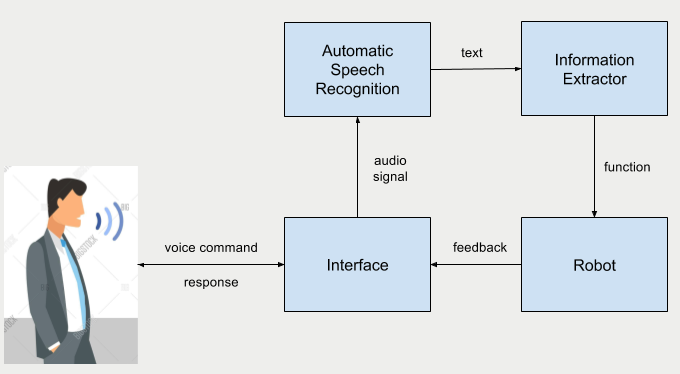
\includegraphics[width = 0.7\hsize]{./figures/diagramSystem}
%	\caption{Diagram of the system}
%	\label{fig:diagramSystem}
%\end{figure}
\addcontentsline{toc}{chapter}{Abstract}


\chapter*{Acknowledgement}
Firstly, I would like to express my sincere gratitude to my supervisor Prof. Jim Cunningham for the continuous support of my individual project and related research, for his patience, motivation, and immense knowledge. His guidance helped me in all the time of my project and writing of this report.
 
I would also like to thank my co-supervisor Prof. Stefan Leutenegger for his insightful advices and comments on my individual project. My sincere thanks also goes to Prof. Marc Deisenroth, Dr. Timothy Kimber, all the members in the Computing Support Group and the Microsoft Azure Grant program who gave access to the laboratory and research facilities. Without their precious support it would not be possible to conduct this project.

Finally, I must express my very profound gratitude to my family for providing me with unfailing support and continuous encouragement throughout my years of study and through the process of doing my project. This accomplishment would not have been possible without them. 

Thank you!

Author\\
Hong Anh VU




\addcontentsline{toc}{chapter}{Acknowledgement}

\chapter{Introduction}
%\begin{figure}[tb]
%\centering
%
\includegraphics[width = 0.4\hsize]{./figures/imperial}
%\caption{Imperial College Logo. It's nice blue, and the font is quite stylish. But you can choose a different one if you don't like it.}
%\label{fig:logo}
%\end{figure}
%
%Figure~\ref{fig:logo} is an example of a figure. 
The rise of voice-based interfaces is really impressive over the last couple of years. They are not only integrated to mobile device (Apple Siri, Google Assitant) but also deployed to entire voice-first device (Amazon Echo, Google Home). According to VoiceLabs's report \cite{VoiceLabs:2017}, there were 1.7 million voice-first devices shipped in 2015. In 2016, this figure were 6.5 million and is predicted to be 24.5 million this year. The potential to build application on top of these interfaces seems limitless. We can directly use voice to order the device to play music, read newspaper, turn on/off light etc. My project is focused on robotic applications, specially for remote movement control and object finding. The general objective is to build a voice system that listens to user's commands, transfers these audio signals to text, extracts the information from text and maps to corresponding robot actions (figure \ref{fig:diagramSystem}). A more ambitious goal is to illustrate an interactive learning process of the robot. This will be tackled during the project.
\begin{figure}[tb]
\centering
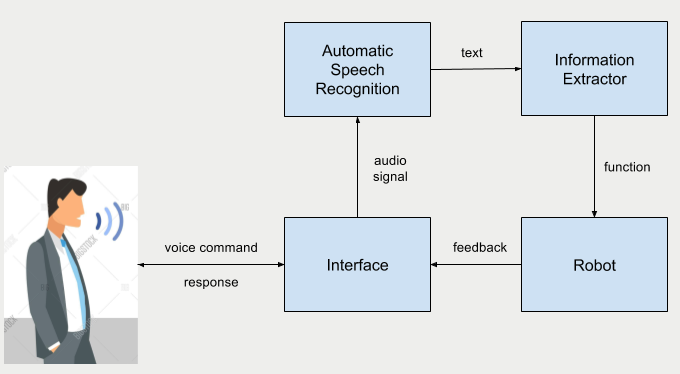
\includegraphics[width = 0.7\hsize]{./figures/diagramSystem}
\caption{Diagram of the system}
\label{fig:diagramSystem}
\end{figure}


%Two closely related reasons for this booming era of voice-based system is the success of Deep Neural Network along with the availibility of Big Data. 
%
%Deep Neural Network (DNN) is a machine learning method that was introduced in second half of 20th century. Because of its massive computation demand, DNN was not successful until 2012, when strong GPU and big data are available. Previously, traditional methods of speech recognition and speech synthesis based on Gaussian Mixture and Hidden Markov models involve many non-uniform internal-handcrafting rules 
%
%have been taken over by DNN

%\chapter{Guideline}
%\newpage
\tbf{Abstract}: The abstract is a very brief summary of the report's contents. It should be about half page long. Somebody unfamiliar with your project should have a good idea of what it is about having read the abstract alone and will know whether it will be of interest to them.\\

\tbf{Acknowledgements}: It is usual to thank those individuals who have provided particularly useful assistance, technical or otherwise, during your project. Your supervisor will obviously be pleased to be acknowledged as they will have invested quite a lot of time overseeing your progress.\\

\tbf{Contents page}: This should list the main chapters and (sub) sections of your report. Choose self-explanatory chapter and section titles. If possible you should include page numbers indicating where each chapter/section begins. Try to avoid too many levels of subheading. Try if possible to stick to sections and subsections; subsubsections are usually avoidable.\\

\tbf{Introduction}: This is one of the most important components of the report. It should begin with a clear statement of what the project is about so that the nature and scope of the project can be understood by the reader. It should summarise everything you set out to achieve, provide a clear summary of the project's background and relevance to other work, and give pointers to the remaining sections of the report that contain the bulk of the technical material.\\

\tbf{Background and related work}: The background and related work section of the report should set the project into context by relating it to existing published work that you read at the start of the project when your approach and methods were being considered. There are usually many ways of approaching a given problem, and you should not just pick one at random. Describe and evaluate as many alternative approaches as possible. The published work may be in the form of research papers, articles, text books, technical manuals, or even existing software or hardware of which you have had hands-on experience. Do not be afraid to acknowledge the sources of your inspiration; you are expected to have seen and thought about other people's ideas, so your contribution largely will be putting them into practice in some other context.\\

\tbf{Body of report}: The central part of the report typically consists of three of four chapters detailing the technical work undertaken during the project. The structure of these chapters is highly project dependent. Usually they reflect the chronological development of the project, e.g., design, implementation, experimentation, and optimisation, although this is not always the best approach. However you choose to structure this part of the report, you should make it clear how you arrived at your chosen approach in preference to the other alternatives documented in the background. For implementation projects you should describe and justify the design of your system at some high level, for example by using any of the design methods taught during the first- and second-term courses, and should document any interesting problems with, or features of, your implementation. Integration and testing are also important to describe. Your supervisor will advise you on the most suitable structure for these middle sections.\\

\tbf{Evaluation:} All projects need to contain a serious and careful evaluation of their results. The specifics of the evaluation method (e.g., user study, experiments, formal proof review, etc.) are intrinsic to the nature of the project, so this is something that you must discuss and agree with your supervisor early in the project. Ideally, a presentation of the method and results of your evaluation should be included in its own separate section of the report.\\

\tbf{Conclusions and future work}: All good projects conclude with an objective evaluation of the project's successes and failures, and suggestions for future work that can take the project further. It is important to understand that there is no such thing as a perfect project. Even the very best pieces of work have their limitations and you are expected to provide a proper critical appraisal of what you have done. Your assessors are bound to spot the limitations of your work and you are expected to be able to do the same.\\

\tbf{Bibliography:} This consists of a list of all the books, articles, manuals, etc., used in the project and referred to in the report. You should provide enough information to allow the reader to find the source. You should give the full title and author, and you should state where it is published, including full issue number, date, and page numbers where necessary. In the case of a text book, you should quote the name of the publisher as well as the author(s).\\

\tbf{Appendices: } Appendices contain information that is peripheral to the main body of the report. Information typically included are things like program listings, tables, proofs, graphs, or any other material that would break up the theme of the text if it appeared in situ. Large program listings are rarely required, and should be compressed as much as possible, e.g., by printing in multiple columns and by using small font sizes, omitting inessential detail.\\

\tbf{User guide: } For projects that result in a new piece of software, you should provide a proper user guide providing easily understood instructions on how to install and use it. A particularly useful approach is to treat the user guide as a walk through of a typical session, or set of sessions, that collectively display all the features of your software. Technical details of how the software works is rarely required. Keep it concise and simple. The extensive use of diagrams illustrating the software in action prove particularly helpful. The user guide is sometimes included as a chapter in the main body of the report, but is often better as an appendix to the main report.\\
%%%%%%%%%%%%%%%%%%%%%%%%%%%%%%%%%%%%
\chapter{Background}

%From diagram \ref{fig:diagramSystem}, my system has four main blocks. This chapter is dedicated to describe functionalities of these components as well as the background behind.
This chapter is dedicated to describe briefly theoretical background as well as alternative solutions to subtasks of the project. We will cover from automatic Speech-To-Text, Information Extraction, to Deep Convolutional Neural Network to classify image etc.

\section{Automatic Speech Recognition system}
Automatic Speech Recognition (ASR) system is the core part in any voice command system. Given the audio input, ASR system will output the text form of the input for later processing. Briefly, the audio input is in form of a sound wave over the recording time. It's sampled at a rate of 16000Hz which is enough for recognition. Then this sound wave is chunked at each 20ms and transformed to a spectrogram by using Fourier transform. This then be feeded to a kind of recurrent neural network \cite{Medium:2016}. The output at each time slot is the characters and we normally have a language model to refine this. 

Note that to build an ASR system that performs at the level of Amazon Alexa or Google Now, we need a lot of training data in both quantity (hundreds of thousands hours of spoken audio) and diversity (native and non-native speakers, with and without background noise, etc.) And this kind of data is not available. As the main objective of the project is to use voice to control the robot, not to build a decent ASR system hence I decided to use existing softwares. I explored two solutions: open source systems and Google Cloud.

\subsection{Open-source ASR}
I tried several open-source softwares such as Kaldi \cite{Kaldi:2017}, CMUSphinx \cite{CMUSphinx:2017} and Deep Speech Nervana \cite{DeepSpeech:2017}. As a non-native speaker, I found that they do not perform at an adequate level. For example, I often get "tune rite" when I say "turn right". In addition, it's not easy to use the libraries because long installation processes are required and proper documentations of their usage are limited.

\subsection{Google Cloud Speech API}
My alternative solution is to use a cloud service Google Speech API \cite{GoogleCloud:2017}. Although the system needs to have internet access, it provides qualitative speech recognition and easy to use: we send the audio content and get back the text. By this, we also cut the computation cost of using an ASR server locally. Note that state of the art ASR systems use deep neural network which requires massive computations and resources. For those reasons, I chose to use Google Speech API in my system.

\section{Neural Network Overview}
Neural network is a key technique behind many artifical intelligent systems today. There were already a lot of research about neural network in late 20th century. However, this method only dominates other methods recently (around 2012) thanks to the availability of large datasets and the capability of powerful computation units (GPUs). This section presents briefly convolutional neural networks which is used to classify image.
\subsection{Fully-connected Neural Network}
A fully connected neural network is a directed graph composed by a input layer, several hidden layers and an output layer. An example is shown in figure \ref{fig:fcNet}: The input data is presented by the input layer (e.g. vector of features of input) and is feeded forward through the network to the output layer which represents the probabilities of input's labels. Between each layers, there are learnable parameters: matrix \textbf{weight $W$} and vector \textbf{bias $b$}. Based on the dimensions of input features, number of classes, and hidden layers' sizes, we can easily determine the dimension of these parameters. 
\begin{figure}[tb]
	\centering
	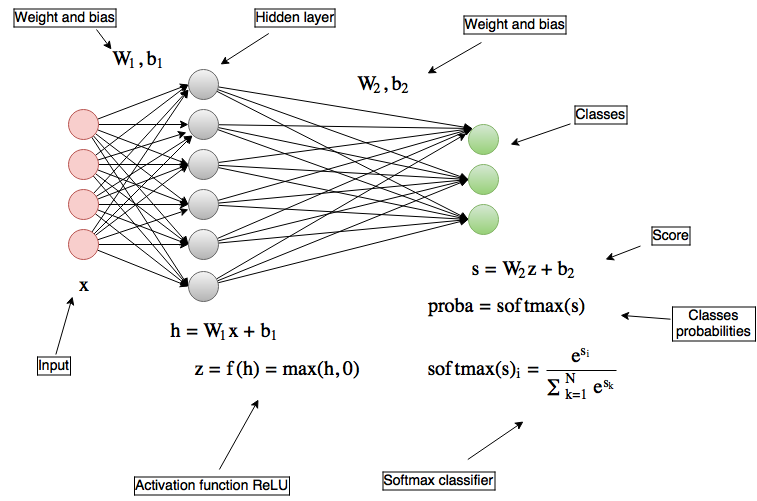
\includegraphics[width=0.9\hsize]{./figures/fcNet}
	\caption{A simple fully connected neural network which classifies an input data into 3 categories using softmax classifier and rectified linear unit activation function (ReLU).}
	\label{fig:fcNet}
\end{figure}
In practice, fully-connected layers are combined with other blocks and they are usually the final block of a classification model. For example, figure \ref{fig:convNet1} shows a simple convolutional neural network with fully-connected layer at the end to classify the input image.
\begin{figure}[tb]
	\centering
	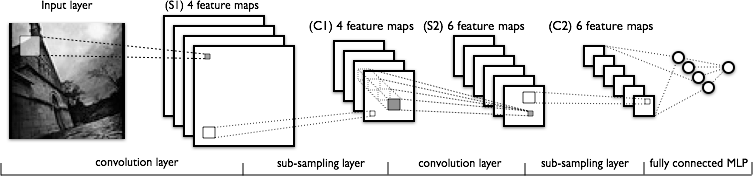
\includegraphics[width=0.9\hsize]{./figures/convNet1}
	\caption{A simple convolutional neural network: its neurons are transposed into 3D shape (width, height and depth) at each layer. The fully connected layer is placed at the end to classify input.}
	\label{fig:convNet1}
\end{figure}
\subsection{Convolutional Neural Network}
Image inputs usually have a 3D shape: width, height and 3 color channels (RGB). Hence, convolutional neural network also aranges its neurons in 3 dimensions: width ($w$), height ($h$), depth ($h$). Note that the depth of input layer equals the number color channels of input image and the \textbf{depth of convolution layer equals the number of filters applied at that layer}. If we use filters of size $3*3$, then in a convolutional layer $i$:
\begin{itemize}
	\item the weight $W_i$ is a stack of filters and $dim(W_i) = 3*3*d_{i-1}*d_i$ where $d_{i-1}$, $d_i$ are depth of layer $i-1$ and $i$ respectively.
	\item the bias $b_i$ is the vector with length equals number of filters, i.e. $b_i \in R^{d_i}$
	\item We convolve the tensor input $w_{i-1}*h_{i-1}*d_{i-1}$ coming from layer $i-1$ with a filter block $3*3*d_{i-1}*d_{i}$ to obtain tensor size $w_{i-1}*h_{i-1}*d_{i}$. Note that we convolve with padding input to keep the same width and height dimension after convolving.
	\item We add bias $b_i$ element-wise for each "surface" (or "slice") $w_{i-1}*h_{i-1}$ of the current tensor.
	\item We apply activation function ReLU to current tensor.
	\item We sub-sample the current tensor to keep strongest features and reduce tensor size. We have final output tensor of size $w_i * h_i *d_i$
\end{itemize}  
The process is illustrated in figure \ref{fig:convNetsimple}. And a common method for sub-sampling called \tbf{max-pooling} shown in figure \ref{fig:maxpool}. It partitions each "slice" of the tensor into non-overlapping rectangles and choose the maximum value in each rectangle. Hence, we produce non-linearities and prioritise strongest features.
\begin{figure}[tb]
	\centering
	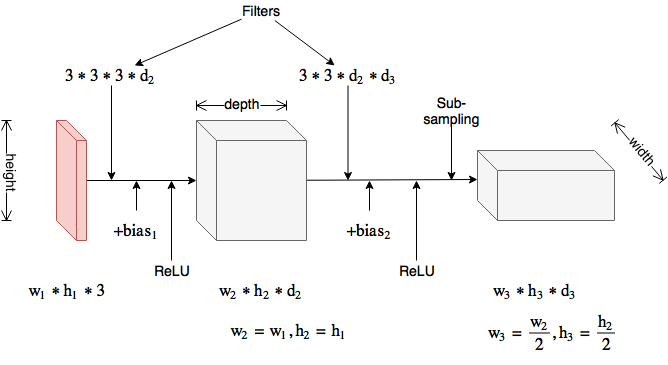
\includegraphics[width=0.9\hsize]{./figures/convNetsimple}
	\caption{Operations and parameters of convolution layers. Note that only input image and 2 convolution layers are drawn here.}
	\label{fig:convNetsimple}
\end{figure}
\begin{figure}[tb]
	\centering
	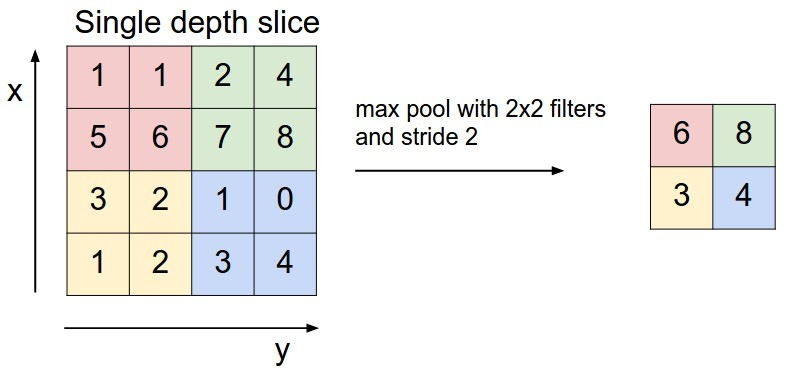
\includegraphics[width=0.6\hsize]{./figures/maxpool}
	\caption{Max-pooling to reduce tensor size and keep strongest features.}
	\label{fig:maxpool}
\end{figure}

After several convolution layers, we flatten the tensor to put into a fully connected neural network for classification. Note that at these fully connected layers, we often use \textbf{dropout} which is a technique to reduce overfitting at fully connected layers because most of parameters present at these layers (figure \ref{fig:dropout}). In training time, we have a probability (normally $p=0.5$) of dropping out neurons in the fully connected layers from the network and then reinsert the dropped out nodes. We repeat that process for every forward and ackward pass. This will also bring a similar effect as model ensemble. In addition, dropout technique can also be used at convolution layers. For more detail about dropout, please refer to \cite{Srivastava:2014:DSW:2627435.2670313}.
\begin{figure}[tb]
	\centering
	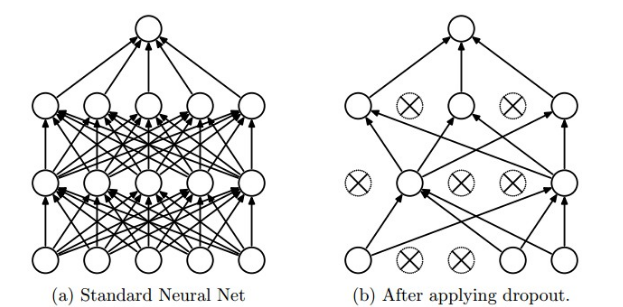
\includegraphics[width=0.8\hsize]{./figures/dropout}
	\caption{Dropout helps to reduce overfitting and ensemble models. Image taken from original paper \cite{Srivastava:2014:DSW:2627435.2670313}.}
	\label{fig:dropout}
\end{figure}

\subsection{Loss Function}
We are left to define a loss function: which allows us to train a machine learning model by updating parameters in order to minimise loss. For classification problems we often use the popular cross-entropy loss function. Consider an input indexed $i$, then its cross-entropy loss is
\begin{align}
\label{form:CELoss}
L_i(s) = -\log(\frac{e^{s_{y_i}}}{\sum_{k=1}^{N}e^{s_k}}) = -s_{y_i} + \log\sum_{k=1}^{N}e^{s_k}
\end{align}
where $y_i$ is its ground-truth label, and $s$ denotes its score at the last layer (see figure \ref{fig:fcNet}). We can see from formula \ref{form:CELoss} that if the score for ground-truth label gets bigger then the loss gets smaller.

Now, given the loss function, we will use stochastic gradient descent to minimise it. There is one hyperparameter related to this optimisation technique which is the learning rate.

\subsection{Train, validate and test}
To train and validate a machine learning model, we usually split the dataset into 3 parts: training set ($\approx56\%$), validation set ($\approx14\%$) and test set ($\approx30\%$). We will use training dataset to train the model (in our case they are all the parameters $W_i$, $b_i$) and use the validation dataset to tune other hyperparameters: learning rates, dropout probability, hidden layer sizes, number of filters etc. Once we have done our best on the validation set, we run a run the model only once on the test dataset and obtain the test accuracy. This figure will be our model performance. 

\section{Image Classification}
\subsection{Overview}
\textbf{Image Classification} is the task of assigning an input image to one label from a fixed set of categories. It's directly related to our object finding problem and we need to solve this first. However, in reality, we are likely to have input image that can contain several objects at once. The related problems are named \textbf{Object Detection} and \textbf{Segmentation}. Image Classification is needed to solve those problems and particularly, if the robot takes images at different view, there might exist the case where only one object is captured and the problem reduces to classify the image. This is not to say that the Image Classification is an easy task. By contrast, this is really hard problem given the following challenges (figure \ref{fig:ImClasschallenges}):
\begin{enumerate}
	\item Viewpoint variation: the same object can be captured at different camera pose.
	\item Illumination conditions: computers only see the pixel values and minor changes in illumination can result in totally different pixel values. 
	\item Scale variation: the same object can have different sizes in the real world. In addition, the distance of taking photo also cause this variation.
	\item Deformation: many objects are not static hence theirs forms are never unique.
	\item Occlusion: depend on the camera view, sometime only a portion of object is visible.
	\item Background clutter: when object and background are similar
	\item intra-class variation: there are many different types and styles of the same object class (e.g. keys, chairs)
\end{enumerate}

\begin{figure}[tb]
\centering
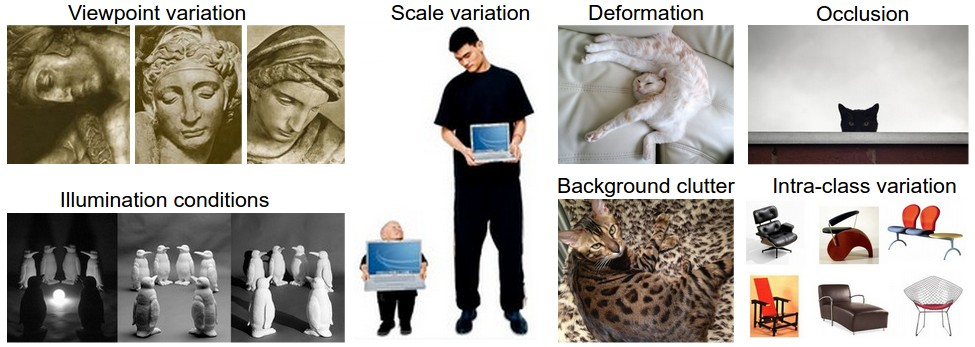
\includegraphics[width =0.9\hsize]{./figures/ImClasschallenges}
\caption{Some challenges of Image Classification problem}
\label{fig:ImClasschallenges}
\end{figure}
\subsection{State-of-the-art Solution}
The family of the best solutions for image classification up to now is deep convolutional neural networks (CNN). Figure \ref{fig:imagenetTop5Err} illustrates this point. Below are some brief explaination for its success:
\begin{itemize}
	\item Deep neural networks accomodate non-linearity properties through activation layers. This makes the system more flexible and able to prioritise important features.
	\item Each convolutional layer is a stack of filters. After learning (i.e. at test time), those filters can extract from input image many types of features such as: edge, shape, colors etc. (for more details see \cite{DeepVis:2015})
	\item Convolutional layers act as features builder, and given enough data, machines do this job better than a human (figure \ref{fig:imagenetTop5Err}).
\end{itemize}


\begin{figure}[tb]
\centering
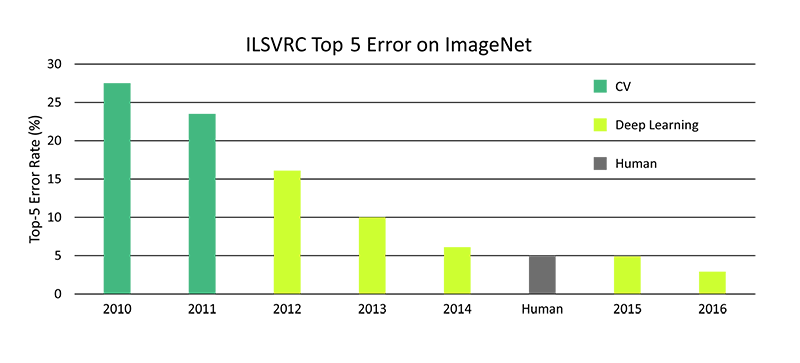
\includegraphics[width=0.9\hsize]{./figures/imagenetTop5Err}
\caption{Top 5 error rate in Imagenet Classification competition from 2010 to 2016. We can note a huge improvement from traditional approaches which use hand-crafted computer vision classifiers (CV) to deep convolutional neural network. VGG model \cite{DBLP:journals/corr/SimonyanZ14a} is the winner in 2014. Its performance nearly equals to human beings.}
\label{fig:imagenetTop5Err}
\end{figure}

\subsection{Transfer Learning from VGG16 model}
To solve my classification problem, I propose to use the VGG16 model \cite{DBLP:journals/corr/SimonyanZ14a} with some modifications at the fully connected layers as we do not have to classify 1000 objects. The original VGG16 model is illustrated in figure \ref{fig:originalVgg16}. Two reasons of using VGG16 model are its good performance and its simplicity compared to other successful models (Microsoft ResNet \cite{DBLP:journals/corr/HeZRS15}, Google Inception \cite{DBLP:journals/corr/SzegedyVISW15}, etc.)
\begin{figure}[tb]
	\centering
	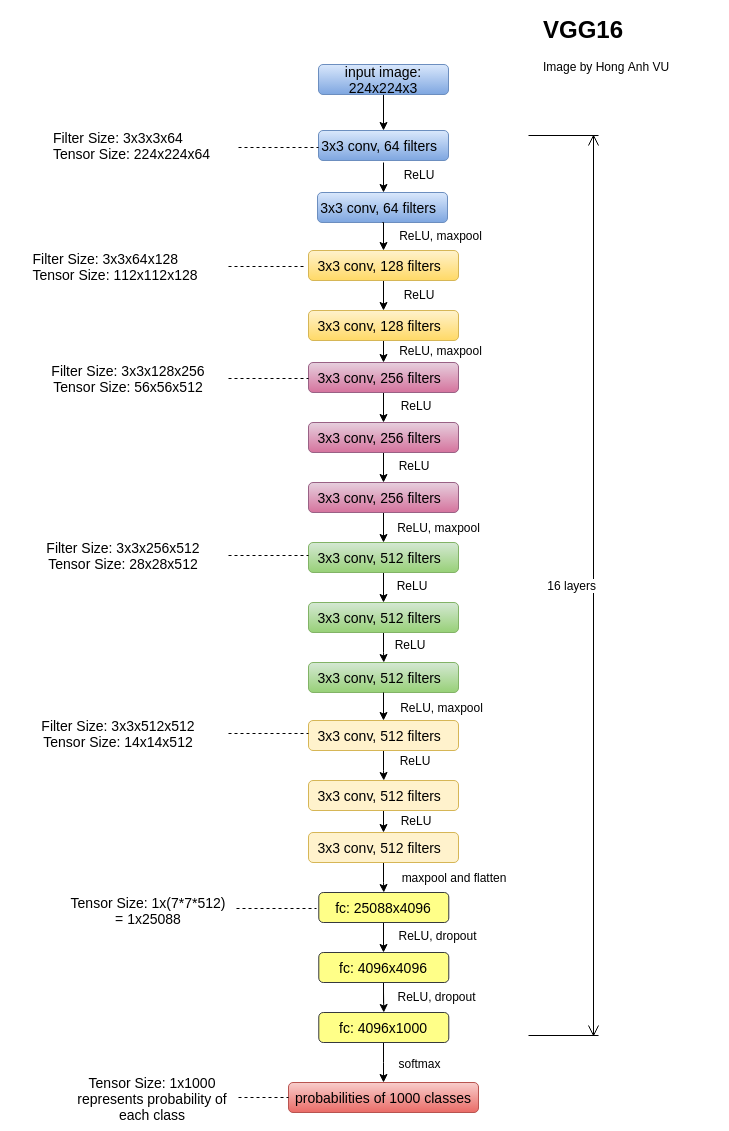
\includegraphics[width=0.9\hsize]{./figures/originalVgg16}
	\caption{Original VGG16 model}
	\label{fig:originalVgg16}
\end{figure}

In my object finding problem, I propose to classify about 12 categories: "apple", "pen", "book", "monitor", "mouse", "wallet", "keyboard", "banana", "key", "mug", "pear", "orange". They are ordinary objects that we see and use daily. To form the dataset, I downloaded 1200 images for each category from ImageNet \cite{imagenet_cvpr09}. In order to solve my problem, I use pretrained weights of convolution layers from original VGG16 model \cite{WeightsVGG:2016} and modify and retrain the fully connected layers (figure \ref{fig:transferedVgg16}). Currently, I obtained a $\approx88\%$ accuracy on test set.
\begin{figure}[tb]
	\centering
	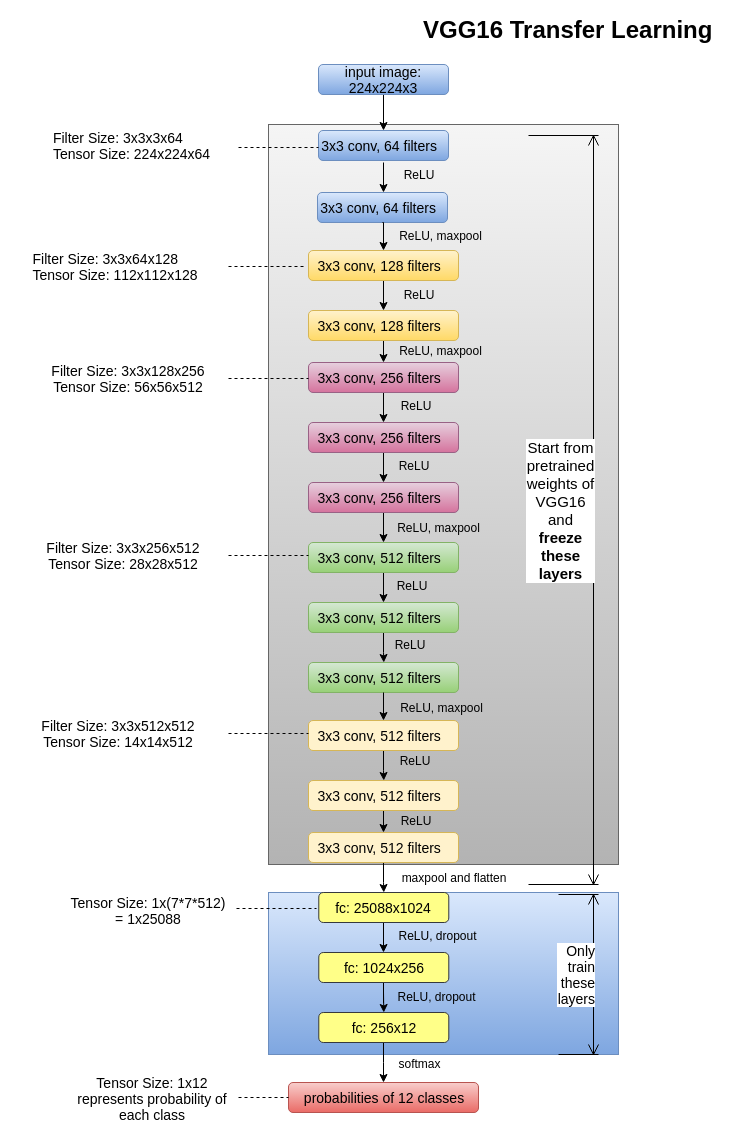
\includegraphics[width=0.9\hsize]{./figures/transferedVgg16}
	\caption{Transfer Learning from VGG16 model}
	\label{fig:transferedVgg16}
\end{figure}

% Example of citation
% Random citation \cite{DUMMY:1} embeddeed in text.
% Another github citation \cite{Johnson2015} is here.

%%%%%%%%%%%%%%%%%%%%%%%%%%%%%%%%%%%%
%\chapter{Progress Summary}  % TO REMOVE in full report
%\section{Current Accomplishment}
The system currently can listen to audio command via a simple GUI interface built on PyQt. This content will be sent to the Google Cloud service to get back the text form. System currently supports 2 intents: forward/backward movement and left/right turn. These actions along with its parameters (angle to turn, distance to move) are analyzed and mapped to program that controls the robot. There is another GUI simulator that draws the movement at the same time. Current setup is illustrated in figure \ref{fig:currentSetup}.
\begin{figure}[tb]
\centering
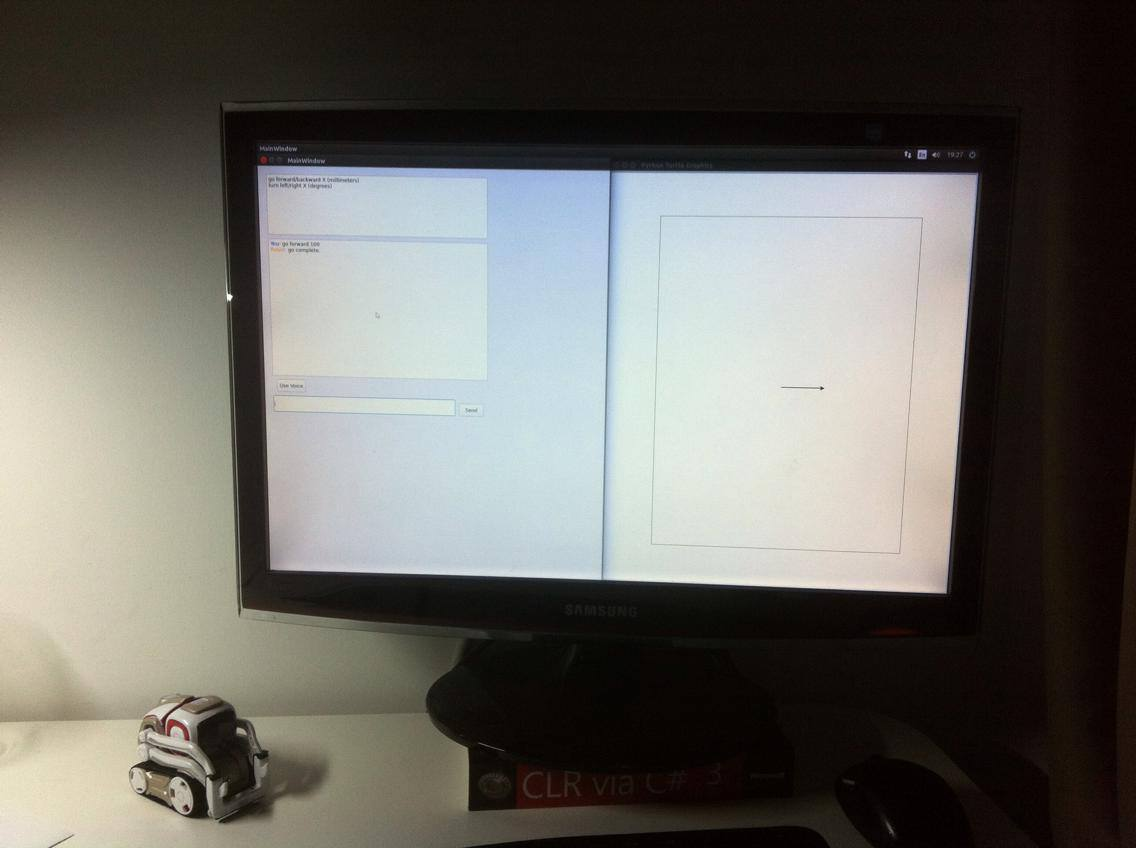
\includegraphics[width = 1.0\hsize]{./figures/currentSetup}
\caption{Current setup of the project: a Cozmo robot (on the left) is connected wirelessly through a mobile device. The program has a simple GUI that can take input in both audio and text formats. Command is analyzed and sent to both robot and a drawing simulator (on the right).}
\label{fig:currentSetup}
\end{figure}

Below is the list of activities to achieve this current state:
\begin{enumerate}
	\item Main Interface:
	\begin{itemize}
		\item Use Python and PyQt to build a simple GUI where the commands can be recorded or typed. It's similar to a chat application between human and robot.
		\item Integrate the GUI with other components of the system: simulator, robot, speech recognition etc.		
	\end{itemize}
	\item Automatic Speech Recognition system:
	\begin{itemize}
		\item Test ASR systems to choose the best one: CMUSphinx, Kaldi, Nervana DeepSpeech, Google Cloud Speech service (the winner)
		\item Signup and Setup Google Cloud client API.
		\item Write code to capture audio input then communicate with Google Cloud service (send request then analyze feedback).		
	\end{itemize}
	\item Information Extractor:
	\begin{itemize}
		\item Attempt to use Part-Of-Speech tags to extract information. However this did not work appropriately in this specific context where commands are spoken, not natural language. 
		\item Apply a set of synonyms to the text input. This eases the processing step: input with specific words corresponds to a unique intent.
		\item Currently, the goal is to build command-oriented system, hence string processing fits well to extract the intent and related parameters.
	\end{itemize}
	\item Robot:
	\begin{itemize}
		\item Search for a robot that can not only fulfill our demands (movement) but also provide other functionalities (built-in camera, built-in speaker, etc.).
		\item In the mean time, build a drawing simulator to test ASR and IE systems.
		\item Get Cozmo robot that fits well with the requirement: it has motors, camera, speaker, LED display, etc. and it's programmable via the SDK \cite{ANKI:2017}.
		\item Install SDK and some other libraries to connect Linux post to the mobile device which controls Cozmo wirelessly.
	\end{itemize}
\end{enumerate}

\section{Problems and Solutions}
\subsection{ASR system}
Firstly, I wanted a open-source and offline solution for the automatic speech recognition system. I tried out several solutions and also thinked of implementing my own ASR system with deep learning. However, there were a few problems for this approach:
\begin{enumerate}
	\item Open-source software for ASR like CMUSphinx \cite{CMUSphinx:2017} and Kaldi \cite{Kaldi:2017} are not good enough. Particularly, they perform quite bad to non-native speakers. And it's not easy to use these libraries.
	\item Build a ASR system from scratch using deep learning is feasible but we will not likely to have a good ASR system. The main reason is the lack of data and powerful ressource for training.
\end{enumerate}
Therefore, I decided to use Google Cloud speech service \cite{GoogleCloud:2017}. It's robust and easy to use: using its API, we send the audio content to the service and get back the text. One trade-off is the internet connection requirement and the system must be authorized to use Google Cloud service. However, it cuts the computation cost if we have a ASR server offline. Note that state of the art ASR system uses deep neural network then requires massive computations.

\subsection{Information Extraction}
Initially, I started processing the text input with the traditional approach where natural language processing tools are used. Given a sentence, I used Part-Of-Speech (POS) tagger to tag each word into categories like verb, nouns, number, adverb, adjective, etc. And based on these tags, I could determine the action (the verb), and its parameters (number, nouns). However, there were a few problems as follow:
\begin{enumerate}
	\item There is no perfect POS tagger and its performance depends on its training data. Hence, it did not show good result in tagging command sentences (which hardly appear in training corpus).
	\item People tend to use short commands such as: "backward X metres", "turn left" (the angle is 90 degree implicitly). Unfortunately, many of these short commands do not compose to a complete sentence. Therefore, POS tagger as well as other natural language processing algorithms can not perform well on incomplete sentence.
	\item The behavior of POS taggers are unpredicted and inconsistent. A minor change in input can lead to total different (and wrong) tags. This does not fit well with voice system where people can make minor grammatical mistakes or paralanguage ("um", "uh" utterances).
\end{enumerate}
Therefore, I switched to use a simpler string processing: 
\begin{enumerate}
	\item First of all, text input will be preprocessed by removing meaningless words like: please, can you, etc.
	\item Secondly, a synonyms set will be applied to replace similar words to its specific key word. 
	\item Finally, a search with some predefined rules is performed to extract the intent and its parameters.
\end{enumerate}
This seems to be more robust (no POStagging) than the first approach. And it fits well with the general goal of this application: say short order and robot acts correspondingly.

\subsection{Main Interface}
The system needs to host interaction between human and robot. Therefore a graphical user interface (GUI) must to be built. It brings numerous advantages: storing the dialogue history, enabling voice-command whenever the user wants by just clicking a button, etc. There are several difficulties:
\begin{enumerate}
	\item Coding up Python GUI application involves using tools as TkInter or PyQt. And learning how to use these libraries takes time.
	\item The system is composed of multiple blocks. In order to have a smooth interface, I need to use threading in some tasks, for example: one thread records voice command, another thread communicates with Google Cloud service, etc. 
\end{enumerate}
All these are technical difficulties and I solved them through many trials and errors.
%%%%%%%%%%%%%%%%%%%%%%%%%%%%%%%%%%%%
%\chapter{Plan}  % TO REMOVE in full report
%The list below describes the remaining tasks and its dedicated time:
\begin{enumerate}
	\item Building object finding system: one of main goals of the project. This involves: \textbf{(1-2 weeks)}
	\begin{enumerate}
		\item Define a set of objects that robot will learn to classify previously.
		\item Prepare the dataset (images) of those objects and train a convolutional neural network for classification.
		\item Based on the classification task, solve the object detection problem. 
		\item After having detected the object, robot needs to automatically move toward and touch it.
	\end{enumerate}
	\item Integrate the object finding system to our main interface. One requirement is that the interface should keep the user a smooth experience of what the robot is doing (e.g. he is searching the object, he is moving toward it). This can be done by both automatically informing and showing the robot's camera. \textbf{(1-2 weeks)}
\end{enumerate}

There are several extensions if we have time:
\begin{enumerate}
	\item Implement text-to-speech system. So human beings can listen to robot's response. \textbf{(1-2 weeks)}
	\item Implement visual-based SLAM system: the robot is placed in a unknown map and it will explore the map. \textbf{(1-2 weeks)}
\end{enumerate}
%The list below describes the remaining tasks and its dedicated time:
\begin{enumerate}
	\item Building object finding system: one of main goals of the project. This involves: \textbf{(1-2 weeks)}
	\begin{enumerate}
		\item Define a set of objects that robot will learn to classify previously.
		\item Prepare the dataset (images) of those objects and train a convolutional neural network for classification.
		\item Based on the classification task, solve the object detection problem. 
		\item After having detected the object, robot needs to automatically move toward and touch it.
	\end{enumerate}
	\item Integrate the object finding system to our main interface. One requirement is that the interface should keep the user a smooth experience of what the robot is doing (e.g. he is searching the object, he is moving toward it). This can be done by both automatically informing and showing the robot's camera. \textbf{(1-2 weeks)}
\end{enumerate}

There are several extensions if we have time:
\begin{enumerate}
	\item Implement text-to-speech system. So human beings can listen to robot's response. \textbf{(1-2 weeks)}
	\item Implement visual-based SLAM system: the robot is placed in a unknown map and it will explore the map. \textbf{(1-2 weeks)}
\end{enumerate}
%%%%%%%%%%%%%%%%%%%%%%%%%%%%%%%%%%%%

\chapter{Implementation}
This chapter describes the user interface as well as some technical details of the implementation of the system. 
\section{User Interface}
The user interface (UI) between the user and the robot appears as a chat application. Figure \ref{fig:chatWindow} illustrates a text box of rules at first, followed by a box of chat dialogue and the message bar. User has 2 ways to interact: either texting or speaking (by using the \tit{Use Voice} button). 
\begin{figure}[tb]
	\centering
	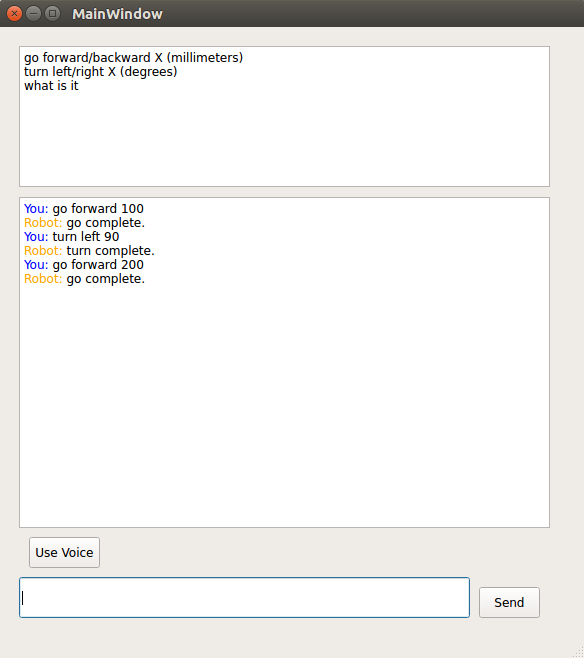
\includegraphics[width=0.8\hsize]{./figures/chatWindow}
	\caption{The chat window of the UI. There is a text box for reminding the rules of commands, followed by a text box of chat dialogue and the message bar.}
	\label{fig:chatWindow}
\end{figure}

The UI is coded using PyQt - one Python binding for Qt cross-platform GUI. The backend behind is Python code because the robot SDK is based on Python3. Beside the real Cozmo robot, I provided a simple robot simulator that can draws the movement commands (figure \ref{fig:simulator}). This simulator is programmed using Turtle module in Python.


\begin{figure}[!htb]
	\centering
	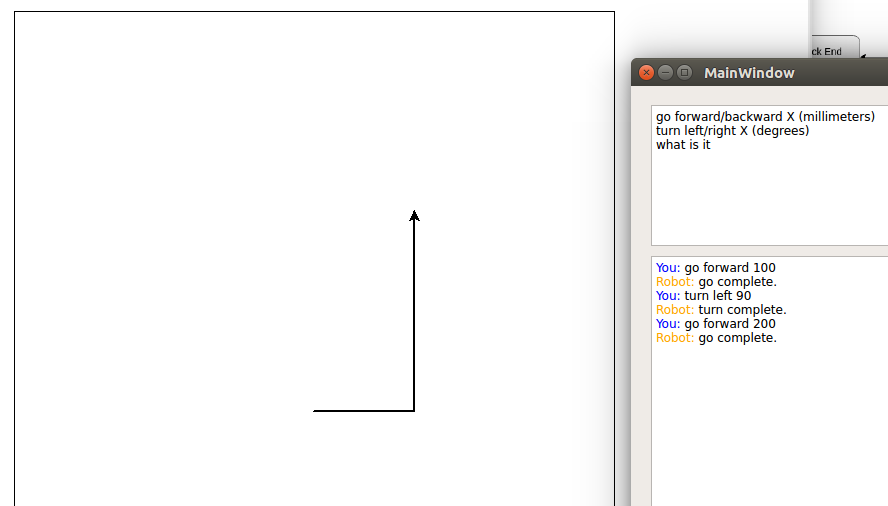
\includegraphics[width=0.8\hsize]{./figures/simulator}
	\caption{Turtle module draws the movement commands. This is useful for testing the system when we don't have a real Cozmo robot.}
	\label{fig:simulator}
\end{figure}

The overview of the system is described in figure \ref{fig:UIdesign}. The left right arrows are used to indicate the interaction between blocks. For example: User sends commands via User Interface and gets responses from here too.

\begin{figure}[!htb]
	\centering
	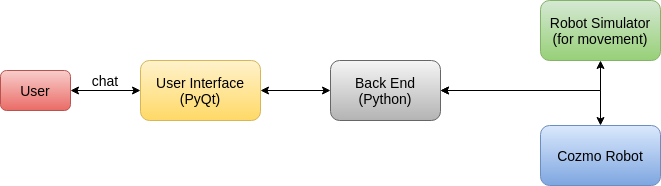
\includegraphics[width=1.0\hsize]{./figures/UIdesign}
	\caption{Overview of the system.}
	\label{fig:UIdesign}
\end{figure}

\section{Cozmo Robot}
\label{sec:Cozmo}
Cozmo (figure \ref{fig:cozmo}) is a great robot produced by Anki \cite{AnkiOfficial:2017}. Beside concise movement ability, it has already a QVGA camera (resolution $320 \times 240$) built-in with frame rate 15fps. Eventhough the camera is not good, it still gives us acceptable images and helps us avoid building a robot from scratch, which can be time consuming. 

\begin{figure}[!htb]
	\centering
	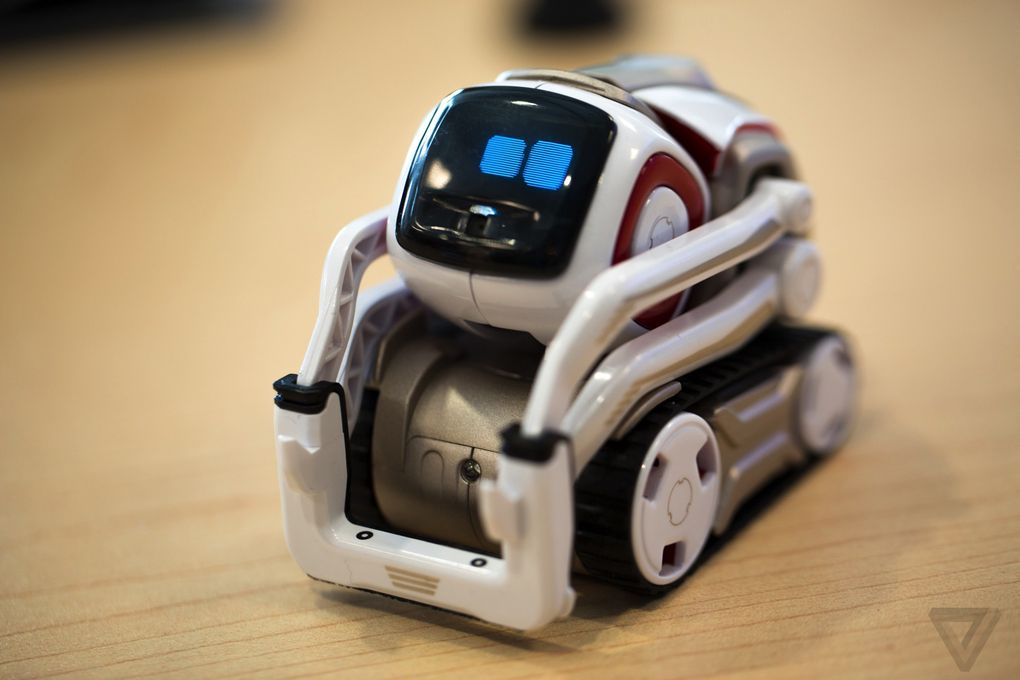
\includegraphics[width=0.8\hsize]{./figures/cozmo}
	\caption{Cozmo robot that has concise movement, built-in QVGA camera as well as other features (LED screen, etc.)}
	\label{fig:cozmo}
\end{figure}


The connection between Cozmo and our system is illustrated in figure \ref{fig:CozmoConnect}. Cozmo will connects to a mobile device (that has Cozmo application installed) via its own wifi. In my setup, the mobile device is an IPad. Then it is connected to our system (the computer) via a USB cable. Linux machines now can access iOS device (such as IPhone, IPad) through \tit{libimobiledevice} \cite{libimobiledevice}. The following steps summarize the process:
\begin{enumerate}
	\item Connect the mobile device to the system via USB.
	\item Start Cozmo and connect the mobile device to the Wifi of Cozmo.
	\item Enable SDK mode in Cozmo application on the mobile device.
	\item Launch our program and start using it.
\end{enumerate}
\begin{figure}[!htb]
	\centering
	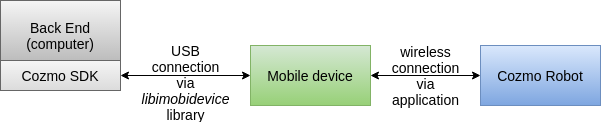
\includegraphics[width=0.9\hsize]{./figures/CozmoConnect}
	\caption{Cozmo connects with the system via a mobile device that has Cozmo app installed.}
	\label{fig:CozmoConnect}
\end{figure}

\section{Reader and Action}
Given the text command, we have a Reader instance that will do the preprocessing and extract information from it (discussed in subsection \ref{sec:InfoExt}). Based on each intents, we map it into an instance of corresponding Action. These Action classes are implemented to control the robot and the simulator to act correspondingly. Figure \ref{fig:readerAction} illustrates this process. 

\begin{figure}[!htb]
	\centering
	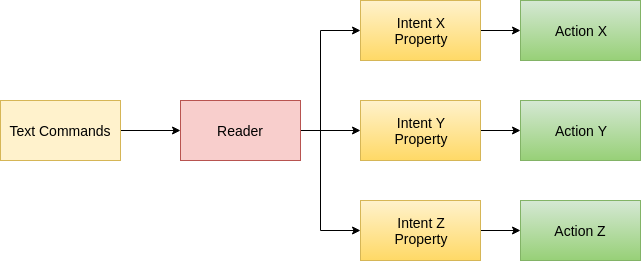
\includegraphics[width=0.9\hsize]{./figures/readerAction}
	\caption{Commands are parsed via a Reader object. Then they are handled accordingly via their corresponding Action objects.}
	\label{fig:readerAction}
\end{figure}


\section{Threading}
There are a few scenarios where we need to use threading in order to avoid freezing the user interface:
\begin{itemize}
	\item time to record the audio command: which can vary from 3 to 15 seconds
	\item speech recognition task that sends audio command over the internet, time for doing this task depends to your inernet connection. However, in practice it's quite fast because the recorded file is about 100Kb.
	\item classify image: ask robot to take a photo, and pass this image through a neural network model (discussed in subsection \ref{sec:transferLearning}) to get prediction of class probabilities.
\end{itemize}

\begin{figure}[!htb]
	\centering
	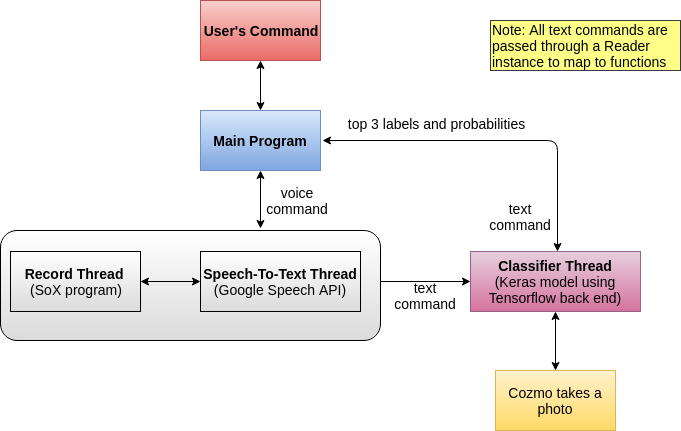
\includegraphics[width=0.9\hsize]{./figures/threads}
	\caption{Threading}
	\label{fig:threads}
\end{figure}

Figure \ref{fig:threads} illustrates the threading structure of the program. Initially, the main program will run these threads in background. Then, whenever user's command needs to use them, these threads are waken up to do their jobs. Note that record thread always works together with speech recognition thread. The idea of seperating them in 2 threads is for further development when we could probably try other speech recognizers.
%%%%%%%%%%%%%%%%%%%%%%%%%%%%%%%%%%%%
%\chapter{Contribution} TODO in full report


%%%%%%%%%%%%%%%%%%%%%%%%%%%%%%%%%%%%
\chapter{Experimental Results}
\label{chap:ExpRes}
Based on sections \ref{sec:neuralNet} and \ref{sec:imgClass}, in this chapter, we will discuss further about the experimental results, particularly of the image classification, distance estimation and object detection problems.

\section{Image Classification}
\label{sec:imgClasEval}
\subsection{Problem Review}
Remember that the problem we are referring in this section is the image classification of images belonging to 12 categories. We have the following details:
\begin{enumerate}
	\item 12 classes: \tit{"apple", "pen", "book", "monitor", "mouse", "wallet", "keyboard", "banana", "key", "mug", "pear", "orange"}.
	\item 1200 images for each class.
	\item Divide the whole dataset into 30\% test set (4320 images), 56\% training set (8064 images) and 14\% validation set (2016 images).
	\item Experiments with multiple options: 
	\begin{itemize}
		\item with/without fine-tuning
		\item with/without image preprocessing
		\item with/without data augmentation
		\item multiple based models (Resnet50, VGG16, Xception)
		\item multiple configuration for fully-connected layer (number of hidden layer, etc.)
	\end{itemize} 
	\item Note that after convolutional block, we flatten the feature tensor to become a 1D feature vector. In addition, our number of classes is fixed to 12. Hence we only denote the hidden layers in the fully-connected part. For example, resnet\_512 is the model uses convolutional blocks of Resnet50 and has fully-connected part as: flatten - 512 - 12. 
	\item Training is done entirely by an Azure NV12 instance which has a GPU Nvidia M60 16GB. Using Resnet50, each epoch takes us $\approx 90$ seconds. We have to train the classifier system $\approx 26$ epochs ($\approx 45 minutes$) to achieve $ > 93\%$ top-1 accuracy.
\end{enumerate}

\subsection{Transfer Learning Result}
\label{sec:transLearnEval}
%\subsection{Results and Observations}
As discussed in subsection \ref{sec:transferLearning}, we can freely design the fully-connected part. After multiple experiments, I found the following interesting observations:
\begin{enumerate}
	\item Bigger fully-connected parts only helps to train the system in fewer epochs. This is reasonable because more complex models has more capacity. However, the trade-off is that we have a bigger model size and it is slower at test time. (figure \ref{fig:compareResnetNoFT})
	\item Fine-tuning the final convolutional block improves the accuracy about 2-3\% (figure \ref{fig:accResnet128NoFT} vs figure \ref{fig:accResnet128})
	\item Image augmentation do not help much in my situation (\ref{fig:compareResnet}). We can see that models with augmented data have better performance in the beginning. However at the end, they are all rougly the same.
	\item As expected, zero-centering and normalization improves a bit the training accuracy (i.e. faster training) but does not improve significantly the validation accuracy. (figures \ref{fig:resnet512StMean}, \ref{fig:accResnet512}, \ref{fig:resnet512StMeanScale}, \ref{fig:accResnet512dup}) I think the reason that it does not improve validation accuracy significantly is the difficulty of our dataset.
	\item Resnet50 is the best base model among VGG16, Xception and Resnet50 (more details are shown in figure \ref{fig:compareModels}). A more carefully fine-tuned version of resnet\_512 model can reach to 94.2\% on validation accuracy.
	\item Accuracy on test set is $\approx$ 93.5\% - 93.7\%. Prediction details can be found in table \ref{table:1}. 
	\item Remark that our dataset is difficult because:
	\begin{itemize}
		\item one image can contain objects of several classes belonging to the 12 categories
		\item the ground truth object does not necessarily appear largely at the center of the image
	\end{itemize}
	Figure \ref{fig:testFail1} and \ref{fig:testFail2} illustrate 2 examples where the system predicts wrongly.
\end{enumerate}
	

\begin{figure}[tb]
	\centering
	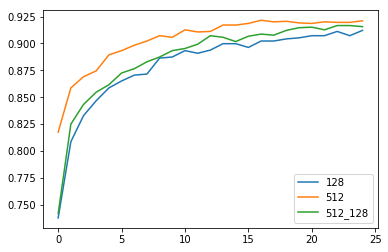
\includegraphics[width=0.6\hsize]{./figures/compareResnetNoFT}
	\caption{Comparison of Resnet models with different fully-connected parts: 128, 512, 512\_128. We can see that bigger model (512) has more capacity and reach the baseline 90\% faster. Multiple layers (512\_128) on the other hand performs worse than one big layer (512).}
	\label{fig:compareResnetNoFT}
\end{figure}

\begin{figure}[!ht]
	\centering
	\begin{minipage}[t]{0.45\linewidth}
		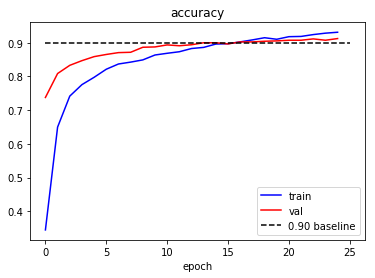
\includegraphics[scale=0.5]{./figures/accResnet128NoFT}
		\caption{resnet\_128 without finetuning: validation accuracy reaches to  $\approx$ 91.6\%}
		\label{fig:accResnet128NoFT}
	\end{minipage}
	\centering
	\begin{minipage}[t]{0.45\linewidth}
		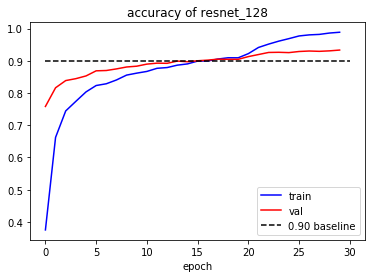
\includegraphics[scale=0.5]{./figures/accResnet128}
		\caption{resnet\_128 fine-tuned around epoch 18: validation accuracy reaches to $\approx$ 93.3\%}
		\label{fig:accResnet128}
	\end{minipage}
\end{figure}


\begin{figure}[tb]
	\centering
	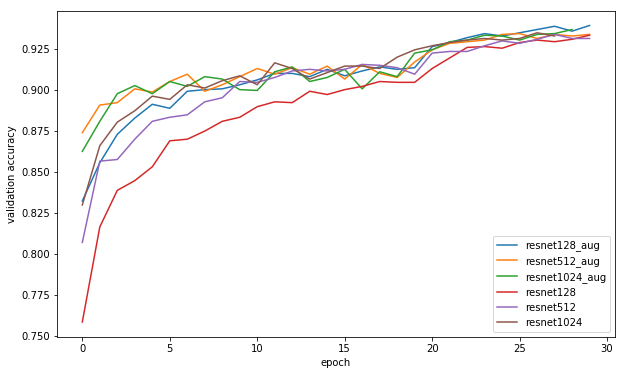
\includegraphics[width=0.8\hsize]{./figures/compareResnet}
	\caption{Comparison of Resnet models with different fully-connected parts: 128, 512, 1024 and with/without data augmentation. We can see that augmentation data does not help much in the end. In the beginning, the accuracy when applying data augmentation is higher because the system is trained on the augmented images (i.e. more training data). Note that all models jumped up around epoch 20 when I applied fine-tuning.}
	\label{fig:compareResnet}
\end{figure}


\begin{figure}[!ht]
	\centering
	\begin{minipage}[t]{0.45\linewidth}
		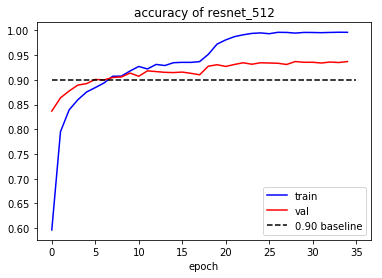
\includegraphics[scale=0.5]{./figures/resnet512StMean}
		\caption{resnet\_512 with mean of training data subtracted. Train accuracy is a bit higher at the beginning.}
		\label{fig:resnet512StMean}
	\end{minipage}
	\centering
	\begin{minipage}[t]{0.45\linewidth}
		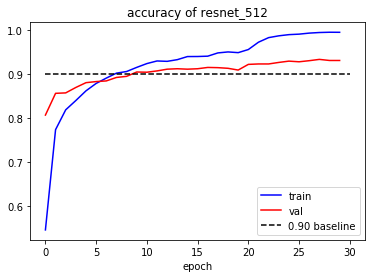
\includegraphics[scale=0.5]{./figures/accResnet512}
		\caption{resnet\_512 with no preprocessing. Both two versions reach $\approx 93.7\%$ validation accuracy at the end.}
		\label{fig:accResnet512}
	\end{minipage}
\end{figure}

\begin{figure}[!ht]
	\centering
	\begin{minipage}[t]{0.45\linewidth}
		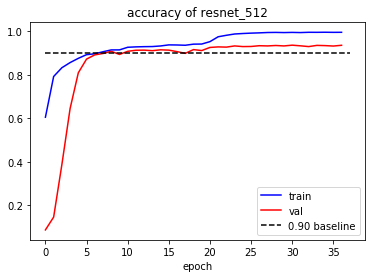
\includegraphics[scale=0.5]{./figures/resnet512StMeanScale}
		\caption{resnet\_512 with both mean of training data subtracted and scaled by dividing to 255. Training is a bit faster but validation accuracy is improving more slowly.}
		\label{fig:resnet512StMeanScale}
	\end{minipage}
	\centering
	\begin{minipage}[t]{0.45\linewidth}
		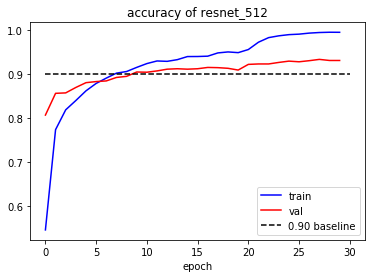
\includegraphics[scale=0.5]{./figures/accResnet512}
		\caption{resnet\_512 with no preprocessing. Both two versions reach $\approx 93.7\%$ validation accuracy at the end.}
		\label{fig:accResnet512dup}
	\end{minipage}
\end{figure}


\begin{figure}[tb]
	\centering
	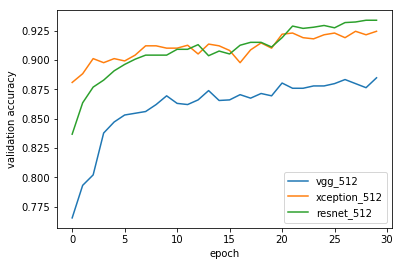
\includegraphics[width=0.7\hsize]{./figures/compareModels}
	\caption{Comparison accross models: VGG16, Resnet50, Xception with the same fully-connected layer (512). We see clearly the model capacity affects the result: VGG16 can not reach base-line 90\% while advanced models like Resnet50 and Xception easily get over 92\%. More precisely, Resnet50 is the best with accuracy greater than $93\%$) and Xception's accuracy is around $92.5\%$.}
	\label{fig:compareModels}
\end{figure}

\begin{figure}[tb]
	\centering
	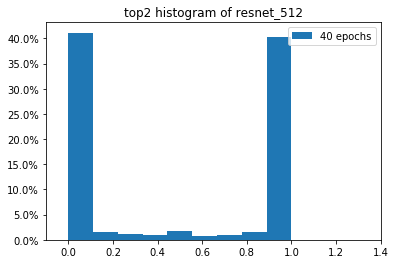
\includegraphics[width=0.6\hsize]{./figures/top2Histo}
	\caption{Histogram of Top 2 predictions probability on test set after training. As expected the trained model is quite sure about its predictions (mostly in $>0.9$ for the maximal probability and $<0.1$ for the second maximal probability). Some samples in the middle represents well the case it is confused due to the difficulty of the dataset.}
	\label{fig:top2Histo}
\end{figure}

\begin{table}[h!]
	\centering
\scriptsize		
	\begin{tabular}{ |c|c|c|c|c|c|c|c|c|c|c|c|c| } 
		\hline
 class &  apple &  pen &  book &  monitor &  mouse &  wallet &  keyboard &  banana &  key &  mug &  pear &  orange \\
 \hline
 apple &  \tbf{0.83} &  0.00 &  0.01 &  0.00 &  0.01 &  0.00 &  0.00 &  0.03 &  0.00 &  0.00 &  0.05 &  0.07 \\
 \hline
 pen &  0.00 &  \tbf{0.96} &  0.00 &  0.00 &  0.01 &  0.01 &  0.00 &  0.00 &  0.01 &  0.00 &  0.00 &  0.00 \\
 \hline
 book &  0.00 &  0.01 &  \tbf{0.96} &  0.01 &  0.00 &  0.02 &  0.00 &  0.00 &  0.00 &  0.00 &  0.00 &  0.00 \\
 \hline
 monitor &  0.00 &  0.01 &  0.01 &  \tbf{0.94} &  0.02 &  0.01 &  0.01 &  0.00 &  0.00 &  0.00 &  0.00 &  0.00 \\
 \hline
 mouse &  0.01 &  0.00 &  0.00 &  0.03 &  \tbf{0.88} &  0.01 &  0.04 &  0.00 &  0.01 &  0.01 &  0.01 &  0.00 \\
 \hline
 wallet &  0.00 &  0.00 &  0.01 &  0.01 &  0.00 &  \tbf{0.96} &  0.00 &  0.00 &  0.02 &  0.00 &  0.00 &  0.00 \\
 \hline
 keyboard &  0.00 &  0.00 &  0.00 &  0.04 &  0.02 &  0.00 &  \tbf{0.94} &  0.00 &  0.00 &  0.00 &  0.00 &  0.00 \\
 \hline
 banana &  0.02 &  0.00 &  0.00 &  0.00 &  0.00 &  0.00 &  0.00 &  \tbf{0.95} &  0.00 &  0.00 &  0.00 &  0.03 \\
 \hline
 key &  0.00 &  0.00 &  0.01 &  0.00 &  0.00 &  0.01 &  0.00 &  0.00 &  \tbf{0.97} &  0.00 &  0.00 &  0.00 \\
 \hline
 mug &  0.00 &  0.00 &  0.00 &  0.00 &  0.00 &  0.00 &  0.00 &  0.01 &  0.00 &  \tbf{0.99} &  0.00 &  0.00 \\
 \hline
 pear &  0.05 &  0.00 &  0.00 &  0.00 &  0.00 &  0.00 &  0.00 &  0.01 &  0.00 &  0.00 &  \tbf{0.91} &  0.02 \\
 \hline
 orange &  0.03 &  0.00 &  0.00 &  0.00 &  0.00 &  0.00 &  0.00 &  0.02 &  0.00 &  0.00 &  0.03 &  \tbf{0.92} \\
 \hline
	\end{tabular}
\caption{Prediction table: each row represents percentage of the system's predictions on the corresponding class. Consider the first row for example: for all images of ground truth \tit{apple}, the systems predicts correctly 83\%, 17\% wrong predictions false mostly to \tit{orange}, \tit{pear}. This is acceptable as noted previously that many fruit images contain objects of mixed classes.}
\label{table:1}
\end{table}

\begin{figure}[!ht]
	\centering
	\begin{minipage}[t]{0.45\linewidth}
		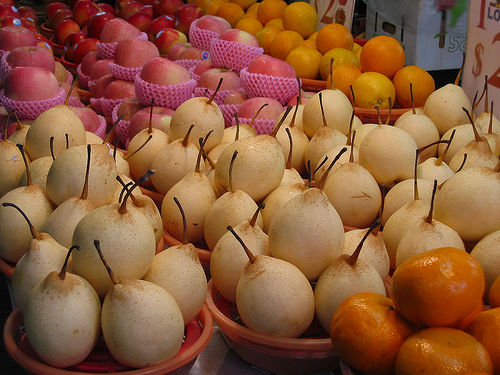
\includegraphics[scale=0.35]{./figures/testFail1}
		\caption{Model predicts \tit{orange} while ground truth is \tit{pear}. We can see that oranges appear in lower right corner and this type of pear is quite special.}
		\label{fig:testFail1}
	\end{minipage}
	\quad
	\begin{minipage}[t]{0.45\linewidth}
		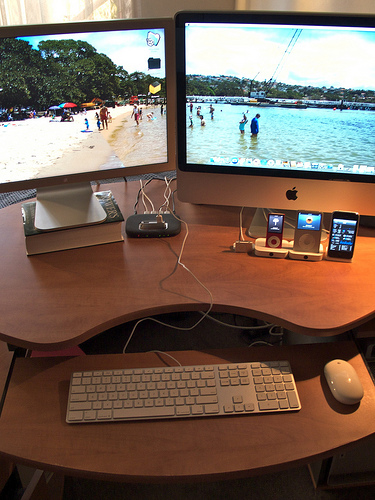
\includegraphics[scale=0.45]{./figures/testFail2}
		\caption{Model predicts \tit{monitor} while ground truth is \tit{keyboard}. We can see 2 bigs monitor in the upper of the image.}
		\label{fig:testFail2}
	\end{minipage}
\end{figure}

\section{Distance Estimation}
\label{sec:distEstimExp}
\subsection{Problem Review}
Distance Estimation is one of the most important task in Robot Localization and Mapping (or Simultaneous Localization and Mapping \cite{wiki:SLAM}). Given the camera's parameters and the size of the object, we can estimate the distance from the camera to the object. The theoretical notions are presented in \ref{sec:camModel}. In this section, we focus on setting up an experiment to verify those notions as well as to quantitatively estimate the order of magnitude of the error.

\subsection{Experiment and Result}
The experiment is setup with the Cozmo robot facing straight ahead a cube. The cube size is 4.4cm (i.e $w = h = 4.4cm$). Remember that all camera parameters are presented in subsection \ref{subsec:camInfo}. The cube is placed at ground truth distance $z \in \{10, 20, 30, 40, 50\}$ (centimeters). Figure \ref{fig:distEstim} illustrates this point. 

\begin{figure}[tb]
	\centering
	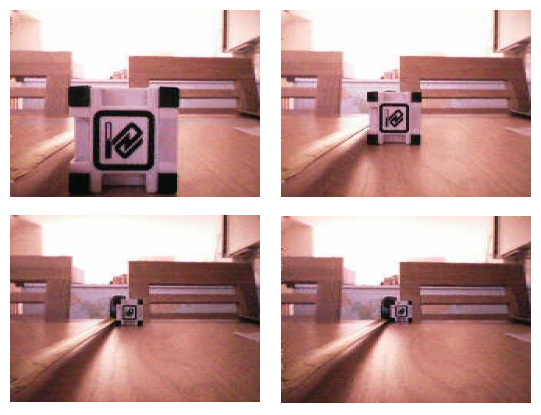
\includegraphics[width=0.6\hsize]{./figures/distEstim}
	\caption{Distance Estimation Experiment: a cube is placed in front of a Cozmo at distances $z = {10, 20, 40, 50}$ centimeters along the $z$ axis. We can see that there is no significant difference between $z = 40$ and $z = 50$ (centimeters). The size of the cube in the image are $w_i \approx {135, 70, 35, 28}$ (pixels) respectively.}
	\label{fig:distEstim}
\end{figure}

Explicitely, we will:
\begin{enumerate}
	\item compute $x_c, y_c, z$ from formula \ref{form:distEst} and \ref{form:centerIm}:
	\begin{align*}
	z = \frac{1}{2} (f_1 \frac{w}{w_i} + f_2 \frac{h}{h_i}) \hspace{0.5cm}
	x_c = \frac{1}{2}\frac{(u_1 + u_2 - 2  c_1)z}{f_1} \hspace{0.5cm} y_c = \frac{1}{2}\frac{(v_1 + v_2 - 2c_2)z}{f_2}
	\end{align*}
	\item compute distance $d$ and verify that $d \approx z$ ($z$ calculated above):
	$$d = \sqrt{x^2 + y^2 + z^2}$$
	\item estimate absolute error $\Delta z$ and relative error $\Delta z / z$ which is close to $\Delta d$ and $\Delta d / d$ respectively since $z \approx d$
\end{enumerate} 

By measuring the corners' coordinates, we obtain $u_1, u_2, v_1, v_2, w_i, h_i$ (in pixels). Knowing also $w = h = 4.4$ (centimeters) together with the camera parameters $f, c_1, c_2$ (in pixels), we can derive from the above formulas the following result:

\begin{table}[h!]
	\centering
	\begin{tabular}{c|c|c|c|c}
ground truth $z$ (cm) & $\hat{z}$ (cm) & $\hat{d}$ (cm) & $\Delta z$ (cm) & $\Delta z / z$ (\%)\\
\hline
\hline
10 & 9.34 & 9.43 & 0.57 & 5.7 \\
\hline
20 & 18.95 & 19.00 & 1.00 & 5.0 \\
\hline
30 & 28.32 & 28.35 & 1.65 & 5.5 \\
\hline
40 & 37.36 & 37.37 & 2.63 & 6.6  \\
\hline
50 & 46.02 & 46.04 & 3.96 & 7.9
	\end{tabular}
	\caption{Distance Estimation Result}
	\label{table:2}
\end{table}

We can see from table \ref{table:2} that:
\begin{itemize} 
	\item $d \approx z$ and have an quantitative estimation about the errors.
	\item The relative error is already $6.5\%$ for this simple setup \tit{where no perspective view error, no bounding box error and no shape variance error are taken into account}. Some examples of these errors will be introduced below. 
	\item In addition, the figures also show the limitation of the camera sensor: for every distance larger than 40 centimeters, we hardly see the cube (of size 4.4 centimeters) in the image (images in second row in figure \ref{fig:distEstim}). 
	\item In my opinion, the range to detect the cube (by a general detector, not accounting the tag on the cube) \tbf{is from 10 to 20 centimeters}. Therefore, a double-size object (of size 8.8 centimeters) are seen in 20 to 40 centimeters. This is quite limited to implement visual based simultaneous localization and mapping (SLAM) algorithm \cite{wiki:SLAM}. Remember that, the more recent Cozmo robots have a better camera sensor: VGA $640 \times 480$ resolution \cite{cozmoTech}. 
\end{itemize}

Based on these observations, we can predict that the order of relative error will be $\geq 10\%$ for a real object when we will take into account:
\begin{enumerate}
	\item variance in size: for example apples have diameter from 5.7 to 8.3 centimeters.
	\item perspective view: for example the handle of a mug can be hidden by the mug itself.
	\item bounding box error: we will see in section \ref{sec:objDetEval} that sometimes the box does not fit 100\% accurately the object. It can be a bit wider or smaller. Such small variances is critical for distance estimation task.
\end{enumerate}
Therefore, implementing a visual-based SLAM system is more reasonably a future work when we have a more recent Cozmo as well as time to implement an adaptive algorithm for distance estimation which makes use of odometry such as Extended Kalman Filter algorithm \cite{wiki:Kalman}.

\section{Object Detection}
\label{sec:objDetEval}
\subsection{Problem Review}
Object Detection is the task of classifying and localizing object(s) inside the given image. The theoretical approach to solve this problem is described in \ref{sec:objDetect}. In this section, we will evaluate our object detection system and also illustrate some results. Please note the following facts below:
\begin{enumerate}
	\item Our dataset is downloaded from ImageNet \cite{imagenet_cvpr09}. It's the same dataset for Image Classification problem. However, the number of samples is much less since not every image is annotated (i.e. no bounding box is provided).
	\item The number of annotated images in our dataset is 4895. Since this is quite small for deep learning algorithms, we will divide the dataset into 4450 training images ($90\%$) and 450 testing images ($10\%$). We can again split the training set into training and validation set, however I decided not to because we do not have time and powerful GPUs to tune the system.
	\item The annotated files are in XML format. I have to write code to parse and preprocess them since some annotations are wrong (bounding box is out of the image boundary, coordinates of top-left corner is bigger than bottom-right corner for example).
	\item The training process is mostly run on \tit{graphic02} workstation in DoC lab (the GPU on that computer is a GTX 1080). Each epoch takes $\approx 2400$ seconds. The system needs to be trained for at least 30 epochs (i.e. 20 hours).
	\item At test time, for each image, detecting and localizing objects take only $\approx 0.4$ second (using \tit{graphic02} workstation).
	\item The base network (i.e. convolutional layers to compute feature vectors) is Resnet50 \cite{DBLP:journals/corr/HeZRS15}. We chose that based on its performance in Image Classification task: both accuracy and speed are impressive.
	\item We also apply transfer learning: we load the pretrained Resnet50 model weight and keep the base network freezed. We only train the top layers such as rpn, classifier and regressor.
	\item We use horizontal flip to augment image.
\end{enumerate}

\subsection{Evaluation}
Table \ref{table:3} shows the Average Precision (AP) measured as well as the number of training and testing images for each class. Below are my observations:
\begin{enumerate}
	\item The overall mean Average Precision (mAP) is $0.619$. In my opinion this is a good result since our dataset is quite small. Normally the number of training images in competitions such as PASCAL VOC \cite{Everingham2010}, ILSVRC \cite{ILSVRC15} is more than $1000$ images for each class.
	\item The class \tit{book} has really small AP: $0.041$. mainly due to two results:
	\begin{itemize}
		\item not enough training and testing data ( $116$ and $12$ respectively)
		\item there are very difficult tests where the book is really small inside the image and sometimes the annotation is either partial or incorrect (figure \ref{fig:bookDifficult}).
	\end{itemize}
	\item The class \tit{pear} has small dataset too, however, images belong to this class are clearer and easier (figure \ref{fig:pear}).
	\item The classes \tit{monitor}, \tit{mouse}, \tit{pen} has low AP due to:
	\begin{itemize}
		\item the images are difficult even for human beings since these objects normally appear together in workplace and there are often a lot of objects there (figure \ref{fig:messyOffice}).
		\item some annotations are partial, i.e. we detect the true object but this can be counted as false positive.
		\item there are similar objects such as wall photo and monitor (figure \ref{fig:similarObj}).
	\end{itemize}
	\item Some True Positive results for ImageNet testset are illustrated in figure \ref{fig:objDetImgNet}.
	\item Some True Positive results for photos taken by Cozmo's camera are illustrated in figure \ref{fig:objDetCozmom}.
	\item Limitations of data from ImageNet are summarized in figure \ref{fig:generalDifficult}: partial, inconsistent and incorrect annotation, "fullscreen" and overlapping objects.
\end{enumerate}

\begin{table}[h!]
	\centering
	\begin{tabular}{c|c|c|c}
		Class & num train & num test & Average Precision \\
		\hline
		\hline
		book & 116 & 12 & 0.041 \\
		\hline
		apple & 409 & 41 & 0.809 \\
		\hline
		pen & 361 & 37 & 0.243 \\
		\hline
		monitor & 240 & 24 & 0.364 \\
		\hline
		mouse & 500 & 50 & 0.372 \\
		\hline
		wallet & 479 & 47 & 0.842 \\
		\hline
		keyboard & 614 & 61 & 0.873 \\
		\hline
		banana & 364 & 36 & 0.683 \\
		\hline
		key & 347 & 35 & 0.704 \\
		\hline
		mug & 425 & 42 & 0.895 \\
		\hline
		pear & 120 & 12 & 0.804 \\
		\hline
		orange & 475 & 48 & 0.799 \\
		\hline
		Total and mAP & 4450 & 445 & 0.619		
	\end{tabular}
	\caption{Object Detection Evaluation on testset of our ImageNet dataset. Please note that \tit{num train} and \tit{num test} stand for number of training and testing images respectively.}
	\label{table:3}
\end{table}
\begin{figure}[tb]
	\centering
	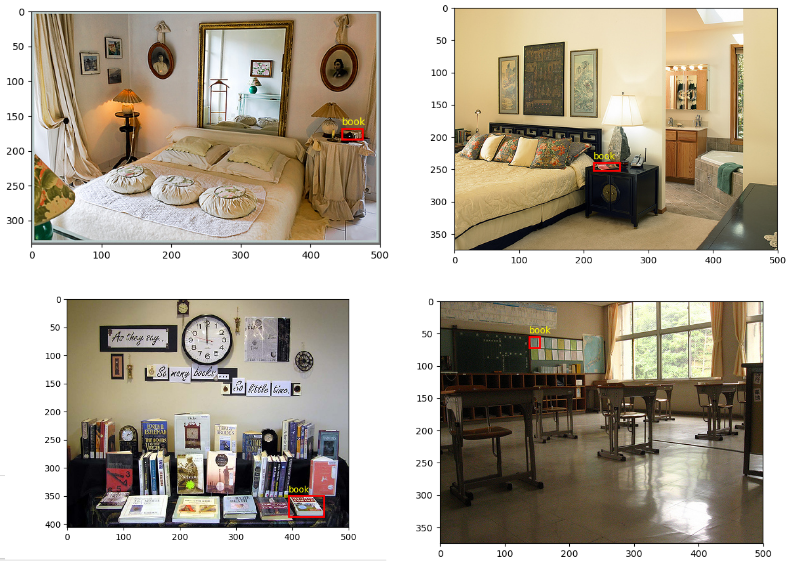
\includegraphics[width=1.0\hsize]{./figures/bookDifficult}
	\caption{The difficulties of detecting books in our ImageNet dataset: the books are really small inside the image (images at higher layer) and sometimes the annotation is either partial (bottom-left image) or incorrect (bottom-right image).}
	\label{fig:bookDifficult}
\end{figure}

\begin{figure}[tb]
	\centering
	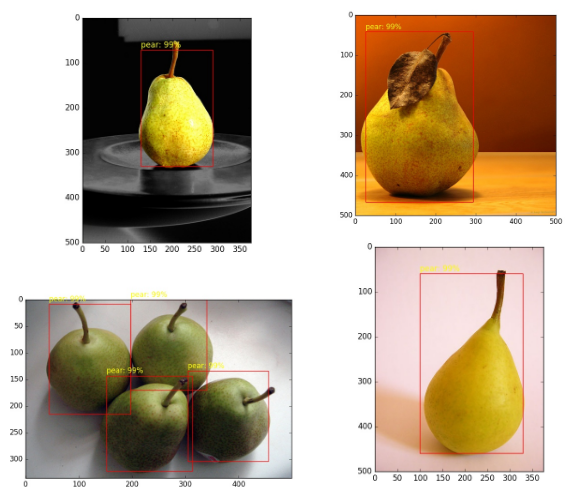
\includegraphics[width=1.0\hsize]{./figures/pear}
	\caption{The class \tit{pear} has small dataset too, however, images belong to this class are clearer and easier. We can see very accurate predictions in the four test images above.}
	\label{fig:pear}
\end{figure}

\begin{figure}[tb]
	\centering
	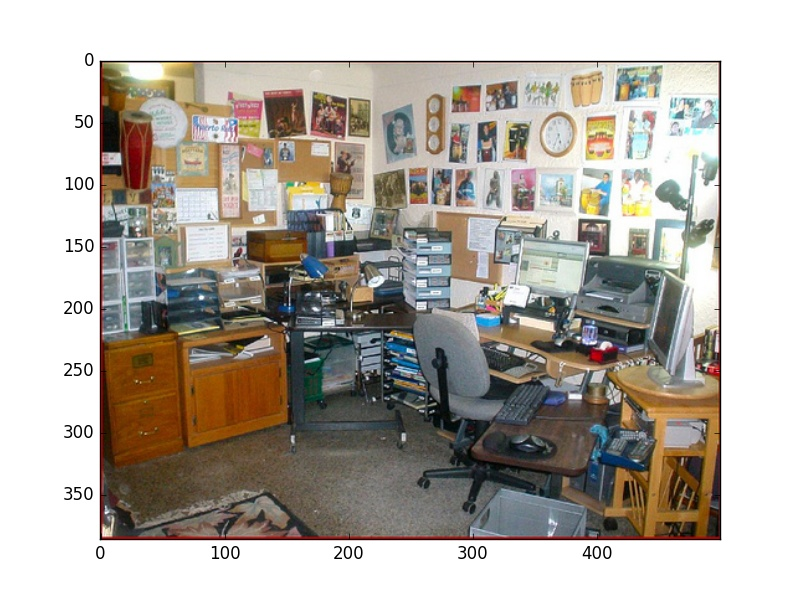
\includegraphics[width=0.8\hsize]{./figures/messyOffice}
	\caption{The objects in 3 classes \tit{monitor}, \tit{mouse}, \tit{pen} often go together in the office place. However, there are offices with a lot of objects.}
	\label{fig:messyOffice}
\end{figure}

\begin{figure}[tb]
	\centering
	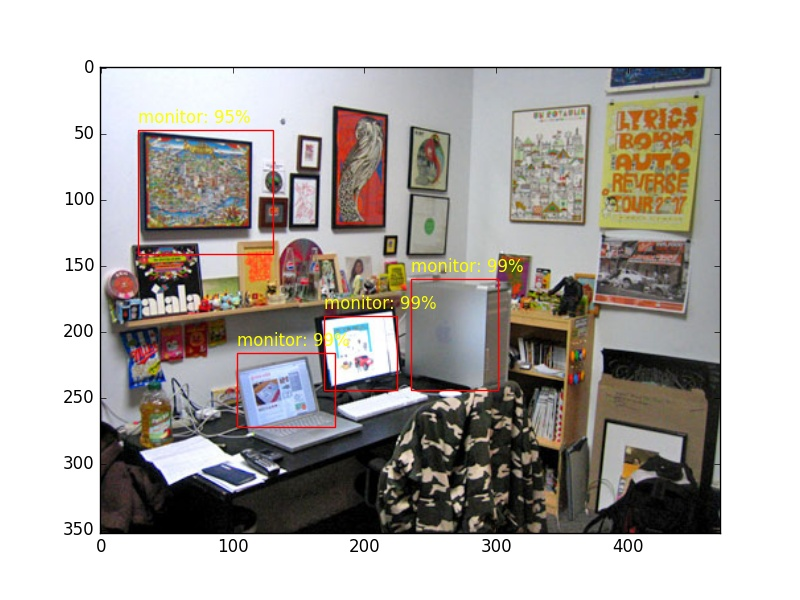
\includegraphics[width=0.8\hsize]{./figures/similarObj}
	\caption{False Positive due to object similarity: wall photo vs monitor.}
	\label{fig:similarObj}
\end{figure}

\begin{figure}[tb]
	\centering
	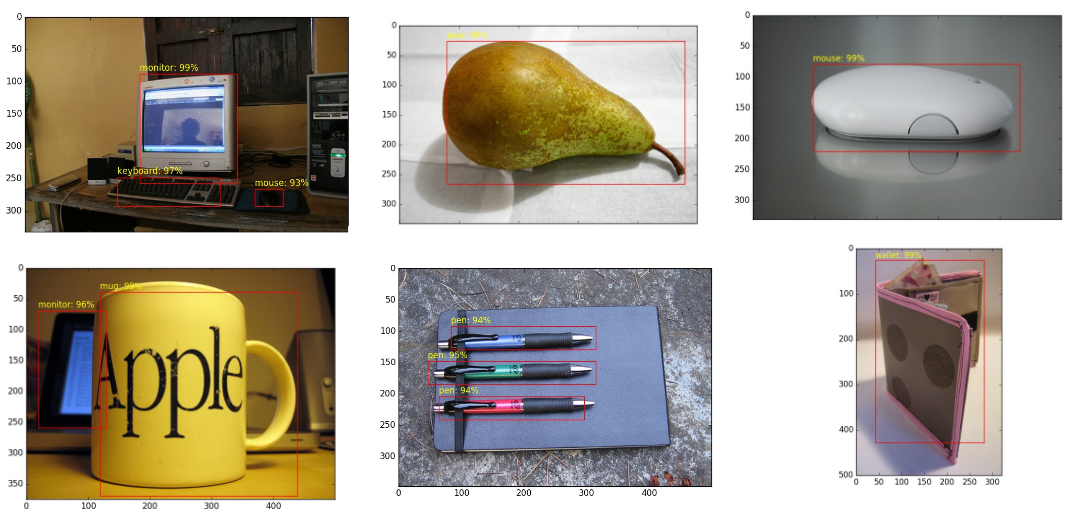
\includegraphics[width=1.0\hsize]{./figures/objDetImgNet}
	\caption{Object Detection with ImageNet: Run our Object Detection System on images in testset from our ImageNet dataset.}
	\label{fig:objDetImgNet}
\end{figure}

\begin{figure}[tb]
	\centering
	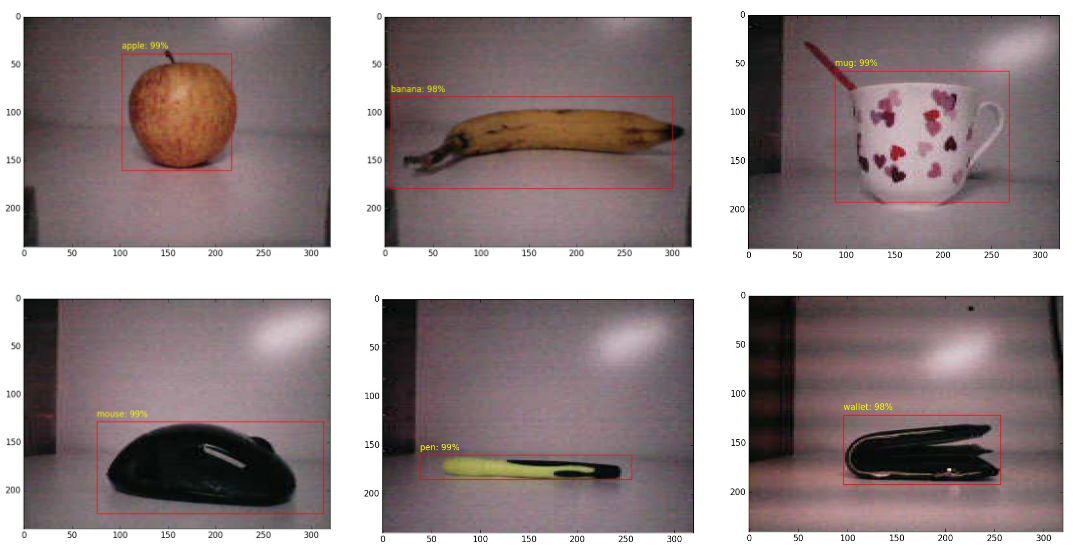
\includegraphics[width=1.0\hsize]{./figures/objDetCozmo}
	\caption{Object Detection with Cozmo's images: Run our Object Detection System on photos taken by Cozmo's camera.}
	\label{fig:objDetCozmom}
\end{figure}

\begin{figure}[tb]
	\centering
	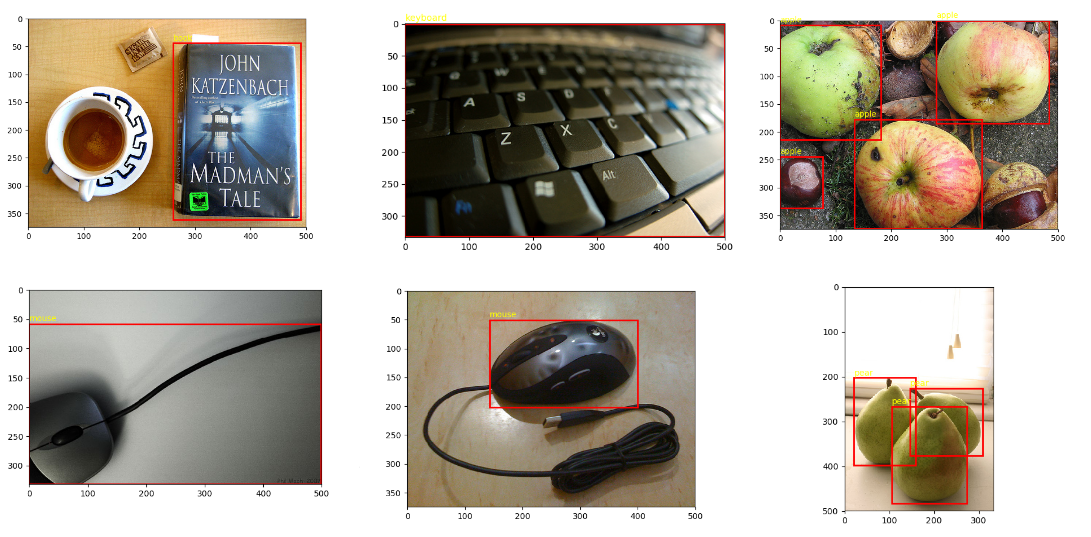
\includegraphics[width=1.0\hsize]{./figures/generalDifficult}
	\caption{Some limitations of ImageNet dataset: partial, inconsistent and incorrect annotation, "fullscreen" and overlapping objects.}
	\label{fig:generalDifficult}
\end{figure}




%%%%%%%%%%%%%%%%%%%%%%%%%%%%%%%%%%%%
\chapter{Conclusions and Future Work}
In conclusion, during a 4-month period, we successfully build a robot application with voice command which:
\begin{itemize}
	\item can order the robot for movement
	\item has integrated with a state-of-the-art neural network image classifier: recognize 12 categories with $> 93\%$ accuracy.
	\item has integrated with a state-of-the-art neural network object detector: detect and localize objects belonging to those 12 categories
	\item can estimate distance of known size object within a range from 20 to 40 centimeters, up to $10\%$ percent error.
\end{itemize}
However, there are a lot of things we can target if we carry on the work:
\begin{enumerate}
	\item the main UI can be more beautiful. In addition, a web interface is also a great idea to share my experience with users that do not have a Cozmo.
	\item implement and embed the visual-based SLAM \cite{wiki:SLAM} using Extended Kalman Filter method \cite{wiki:Kalman}. 
	\item prepare more data (manually annotate images) to get a larger dataset size in order to increase the accuracy of object detection system.
	\item build a robot ourselve which let us choose a good camera since the major part of our application is visual-based.
\end{enumerate}

%% bibliography
%\cleardoublepage
\phantomsection
%\bibliographystyle{apa}
\newpage
\addcontentsline{toc}{chapter}{Bibliography} 
%\bibliographystyle{apa}
\bibliographystyle{abbrv}
\bibliography{mybiblio}

\end{document}
